
\documentclass[12pt]{article}
\usepackage{fontspec}
\usepackage{titlesec}
\usepackage{parskip}
\usepackage[font=small,labelfont=bf]{caption, subcaption}
\usepackage{float}
\usepackage{natbib}
\usepackage{hyperref}
\usepackage{tabu}
\usepackage{setspace}
\usepackage{multirow}
\usepackage{amsmath}
\usepackage{booktabs}
\usepackage[table,xcdraw]{xcolor}
\usepackage{xcolor,colortbl}
\usepackage{lscape}
\usepackage{rotating}
\usepackage{epstopdf}
\usepackage{lineno,xcolor}
\usepackage{ifpdf}
\usepackage{pdflscape}




\hypersetup{
    colorlinks,
    linkcolor={red!50!black},
    citecolor={blue!50!black},
    urlcolor={blue!80!black}
}

\ifpdf 
    \usepackage[pdftex]{graphicx}   % to include graphics
    \pdfcompresslevel=9 
    \usepackage[pdftex,     % sets up hyperref to use pdftex driver
            plainpages=false,   % allows page i and 1 to exist in the same document
            breaklinks=true,    % link texts can be broken at the end of line
            colorlinks=true,
            pdftitle=My Document
            pdfauthor=My Good Self
           ]{hyperref} 
    \usepackage{thumbpdf}
\else 
    \usepackage{graphicx}       % to include graphics
    \usepackage{hyperref}       % to simplify the use of \href
\fi 

\setlength\linenumbersep{5pt}
\renewcommand\linenumberfont{\normalfont\tiny\sffamily\color{gray}}
\makeatletter
\def\ttl@mkchap@i#1#2#3#4#5#6#7{%
  \ttl@assign\@tempskipa#3\relax\beforetitleunit
  %\vspace*{\@tempskipa}% NEW
  \global\@afterindenttrue
  \ifcase#5 \global\@afterindentfalse\fi
  \ttl@assign\@tempskipb#4\relax\aftertitleunit
  \ttl@topmode{\@tempskipb}{%
    \ttl@select{#6}{#1}{#2}{#7}}%
  \ttl@finmarks  % Outside the box!
  \@ifundefined{ttlp@#6}{}{\ttlp@write{#6}}}
\makeatother

\titleformat{\chapter}[display]
    {\huge\bfseries}
    {\Large\chaptertitlename\ \thechapter}
    {0in}
    {}
\titlespacing*{\chapter}{0pt}{*0}{*0}

\setmainfont{Helvetica Neue Light}
\setlength{\parskip}{.5cm}

\usepackage[a4paper,left=2cm, right=2cm, top=2cm, bottom=2cm]{geometry}\usepackage{setspace}
\renewcommand{\baselinestretch}{1.5}

\newcommand\gridfig[2]{%
  \captionof*{subfigure}{}
  \includegraphics[width=5.8cm]{#1}
  \captionof{subfigure}{}\label{#2}%
}

\renewcommand{\bibname}{References}

\newfloat{eqfloat}{h}{eqflts}
\floatname{eqfloat}{Equation}

\author{Sam Brooke\\
  Department of Earth Science \& Engineering\\
  Imperial College London\\ 
  United Kingdom \\
  \texttt{sbrooke@tuta.io}\\
  \href{https://github.com/hijinks/spectral-point}{github.com/hijinks/spectral-point}}
   }
\date{\today}

\newcounter{tmp}

\title{\Huge\texttt{Spectral Point}\\\Large{Version 0.5}\\\vspace{2em}\textit{\normalsize{An application to rapidly collect pixel information\\ from Landsat 8 multispectral imagery}}}

\begin{document}
\maketitle

\newpage

\section{Brief}

\subsection{Google Earth Engine}

Google Earth Engine (GEE) is a cloud-based browser platform that leverages Google’s high-performance computing infrastructure to process large geospatial datasets \citep{Gorelick2017}. The GEE platform is equipped with publicly available high-resolution aerial imagery, digital elevation models and the entire Landsat, Sentinel-1 and Sentinel-2 archive. The GEE code-editor with its Python or JavaScript API allows for production of simple scripts to fully-fledged graphical interfaces in the form of a browser-based web application \citep{Gorelick2017}.

This documentation will guide you through the application of the javascript application \textit{Spectral Point}, built in the GEE development environment. This application provides a simple user interface to select multispectral bands, perform principal component analysis and export point data to a user's Google Drive.

\subsection{Purpose}

\textit{Spectral Point} is run in a single browser window within the Earth Engine development environment \citep{Gorelick2017}, \href{https://code.earthengine.google.com}{code.earthengine.google.com}. As such, the application requires a registered account with Google and a modern web browser. Any data collected in \textit{Spectral Point} will also be exported to the user's Google Drive cloud storage found at \href{https://drive.google.com}{drive.google.com}.

The GEE application \textit{Spectral Point} accomplishes the following workflow;

\begin{itemize}
  \item Selection of Landsat 8 TOA imagery by date or as a cloud-free composite
  \item Selection of a region of interest (ROI) for contrast enhancement
  \item Balance contrast enhancement technique (BCET) image processing
  \item Generation of RGB composites with export capability
  \item Point selection for gathering multiple spectral profiles
  \item Export of location and spectral information
\end{itemize}

\vspace{2em}
\fbox{\begin{minipage}{\textwidth}
The latest version of \textit{Spectral Point} can be found at
\href{https://github.com/hijinks/spectral-point}{github.com/hijinks/spectral-point}\\
The code is licensed under the GNU Lesser General Public License v3.0 and subject to the Google 
Earth Engine terms of service (See \href{https://earthengine.google.com/terms/}{earthengine.google.com/terms/})
\end{minipage}}

\subsection{Interface}

The GEE environment provides an effective means to develop applications that tap into the power of cloud-based processing provided by Google to process rich geospatial datasets in conjunction with easy to edit code and a library to create an user-friendly interface. The interface in \textit{Spectral Point} consists of several steps that begin with choosing a Landsat 8 or Sentinel 2 dataset for exploration, choosing a region of interest or ROI, visualing layers and finally selecting geographic locations to collect data. The typical workspace of the GEE environment can be seen in figure~\ref{fig:workspace_fig}.


\vspace{2em}
\fbox{\begin{minipage}{\textwidth}
\textbf{Note: } This tutorial will focus on processing Landsat 8 imagery only as the Sentinel 2 data is less easily visualised and has fewer in-built libraries in GEE, e.g. cloud-free composite generation. Whilst Sentinel 2 data is available to load into \textit{Spectral Point}, it does not automatically adjust to a visible contrast setting and any imagery does not extent outside the initial map view extent.
\end{minipage}}

\begin{landscape}
\begin{figure}[htbp]
\centering
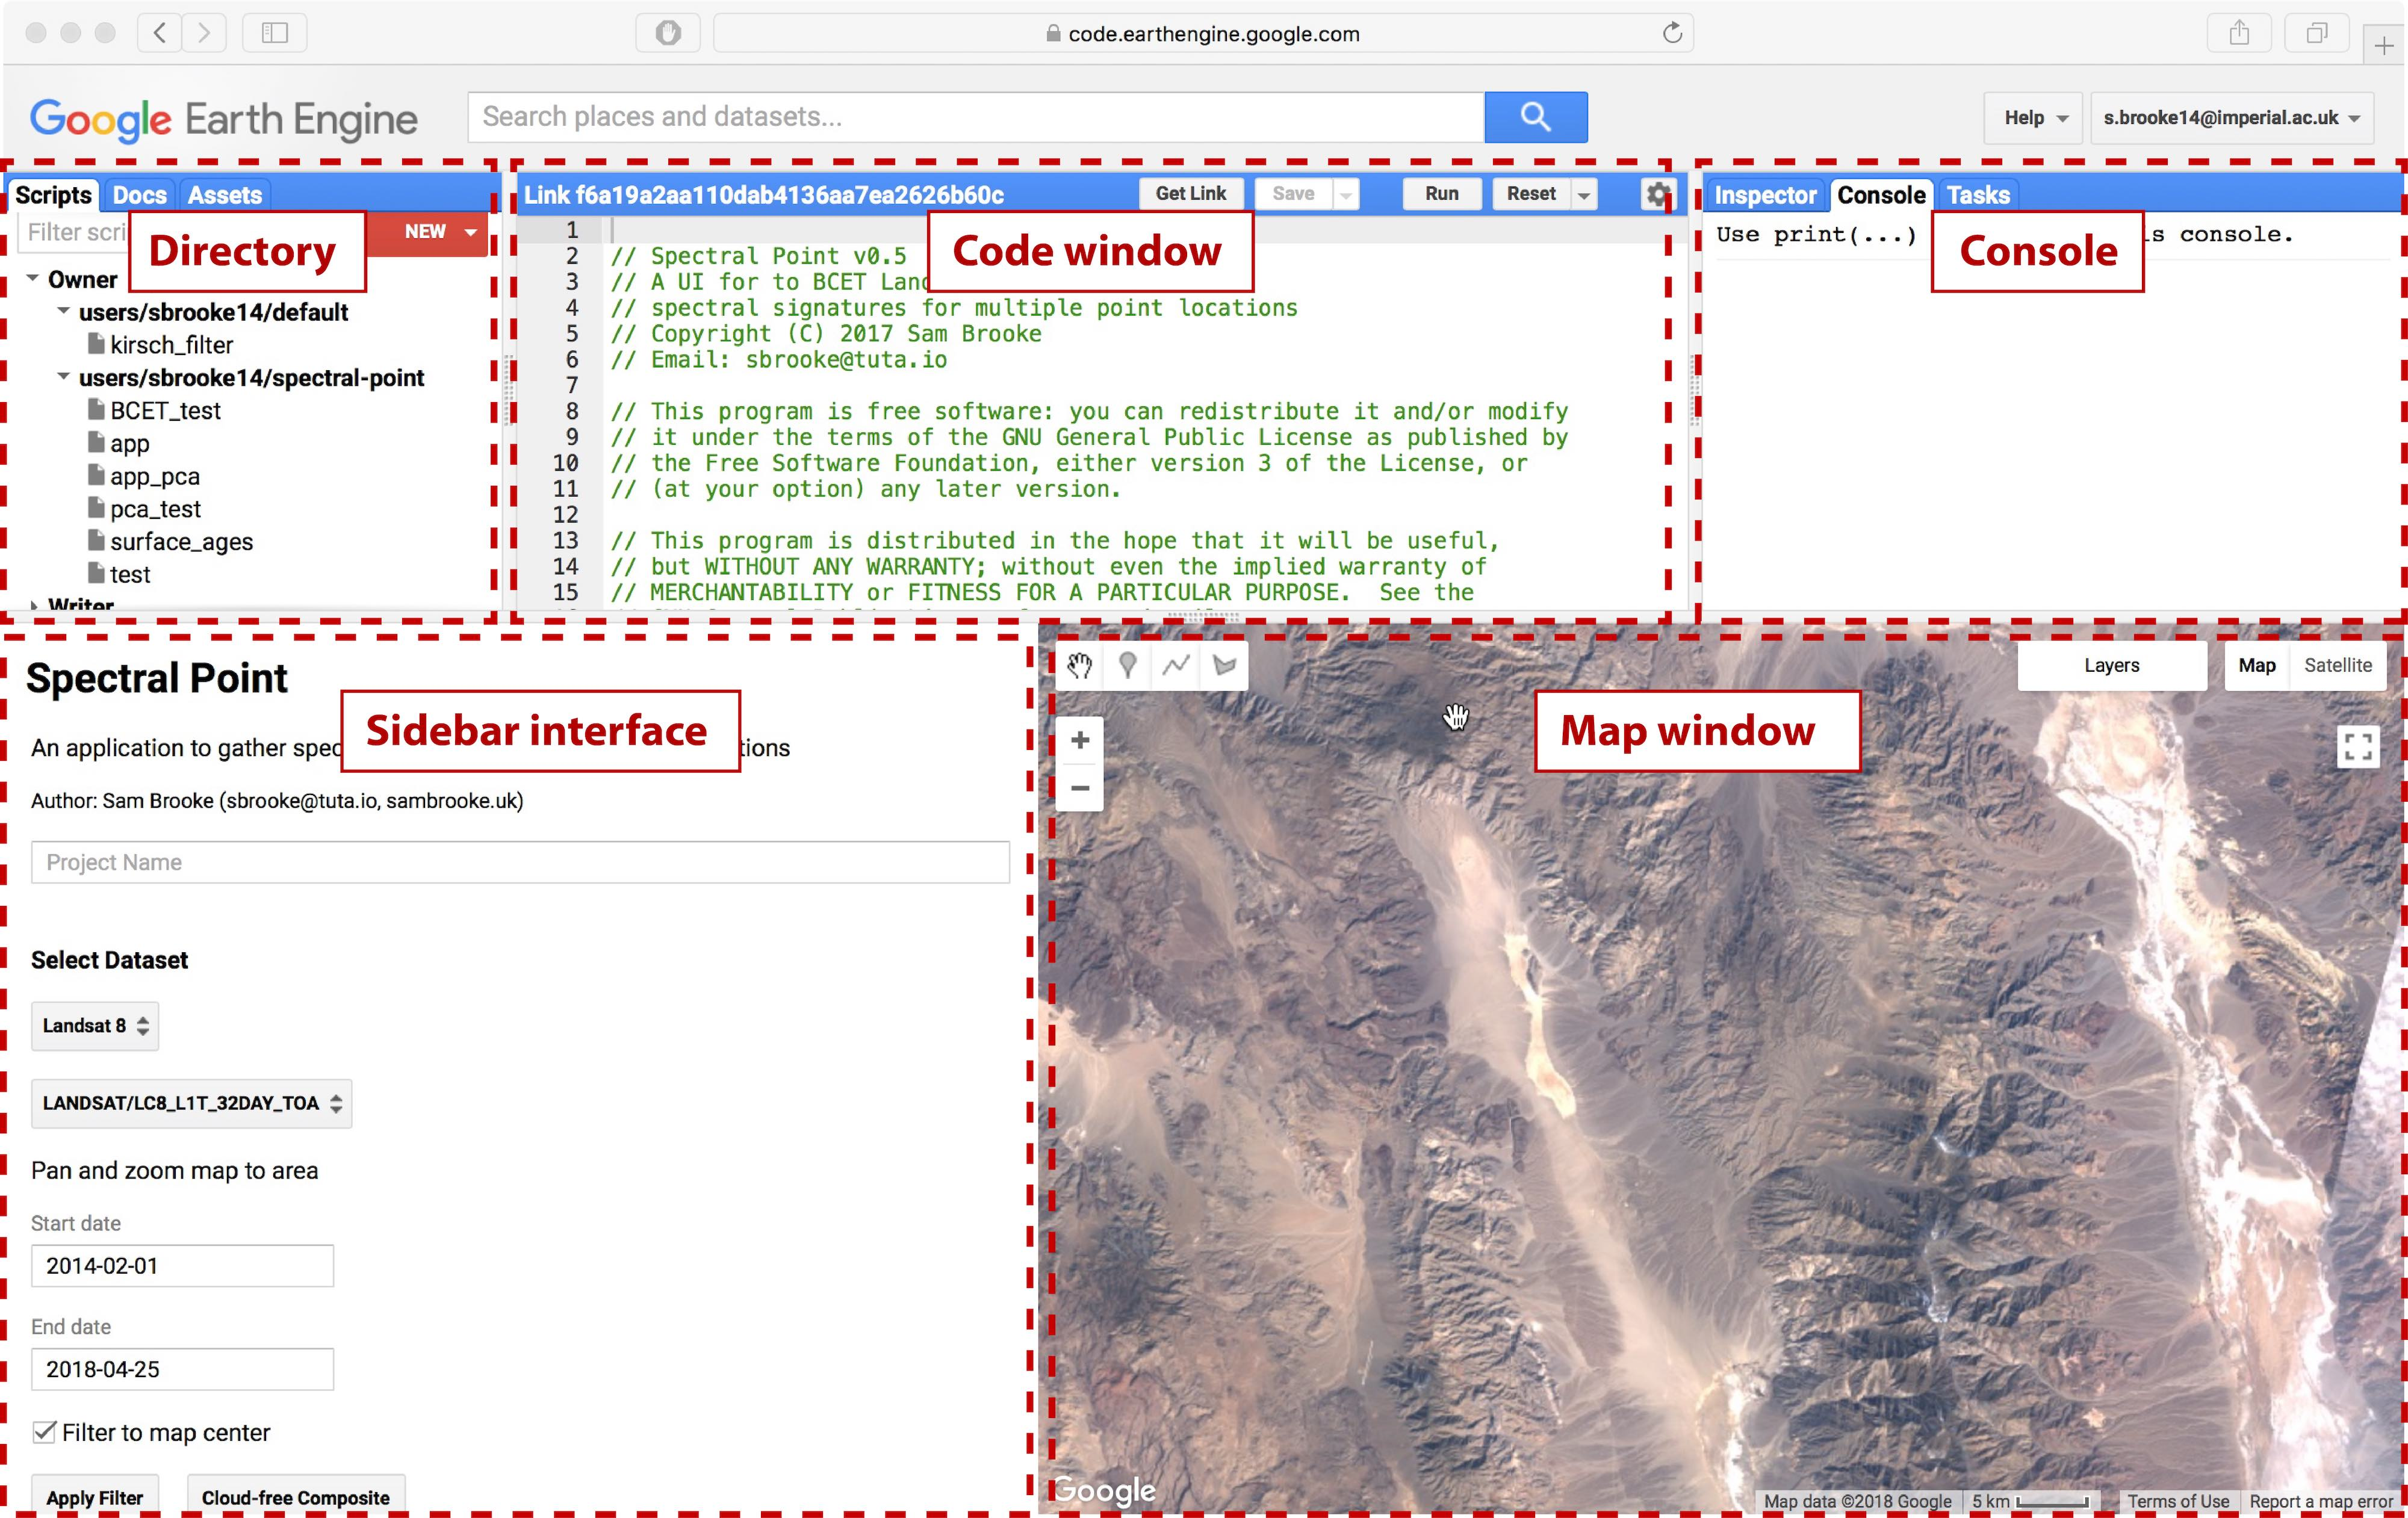
\includegraphics[width=1.2\textwidth]{images/workspace_fig_reduced.jpg}
\caption{The Google Earth Engine development and application environment, available once a Google account is registered with GEE. Key areas are outlined with red dashed boxes, with the top left area showing the user directory, where scripts are organised into files and folders, with tabs to view example scripts, assets and API documentation. The top central area is where code can be viewed, edited and run. The ``Get link'' button provides the capability to generate a version-controlled link to the present state of the script. The top right area is the console, where code outputs are printed within the ``console'' tab and tasks are stored ready for execution in the ``tasks'' tab (See section~\ref{export-data}). The bottom areas are the product of the current script, with a GUI interface that the user can use to navigate the application on the left, and the map viewport on the right. The map area contains tools for navigating viewing extent, adding polygons and manipulating layers.}
\label{fig:workspace_fig}
\end{figure}
\end{landscape}

\section{Selecting a scene}

Using the GEE development environment, all maps are accessible and simple to explore in the adjacent interactive viewport, akin to other Google mapping platforms, with tools to pan, zoom and alter layer visualisation by default (Figure~\ref{fig:layer_visualisation}). The first interface to appear when \textit{Spectral Point} is run (Figure~\ref{fig:choose_imagery}) allows the selection of Landsat 8 TOA imagery based on either premade 16 or 32-day composites between two dates, enabling the user to find the most suitable scene without cloud obstruction or in the desired time of year. A cloud-free composite can also be produced using a cloud scoring algorithm that selects the least-cloudy pixel for a range of Landsat images to develop a new composite raster. All imagery in \textit{Spectral Point} is projected in the EPSG:4326 coordinate system with WGS84 referenced coordinates.

\vspace{2em}
\begin{figure}[htbp]
\centering
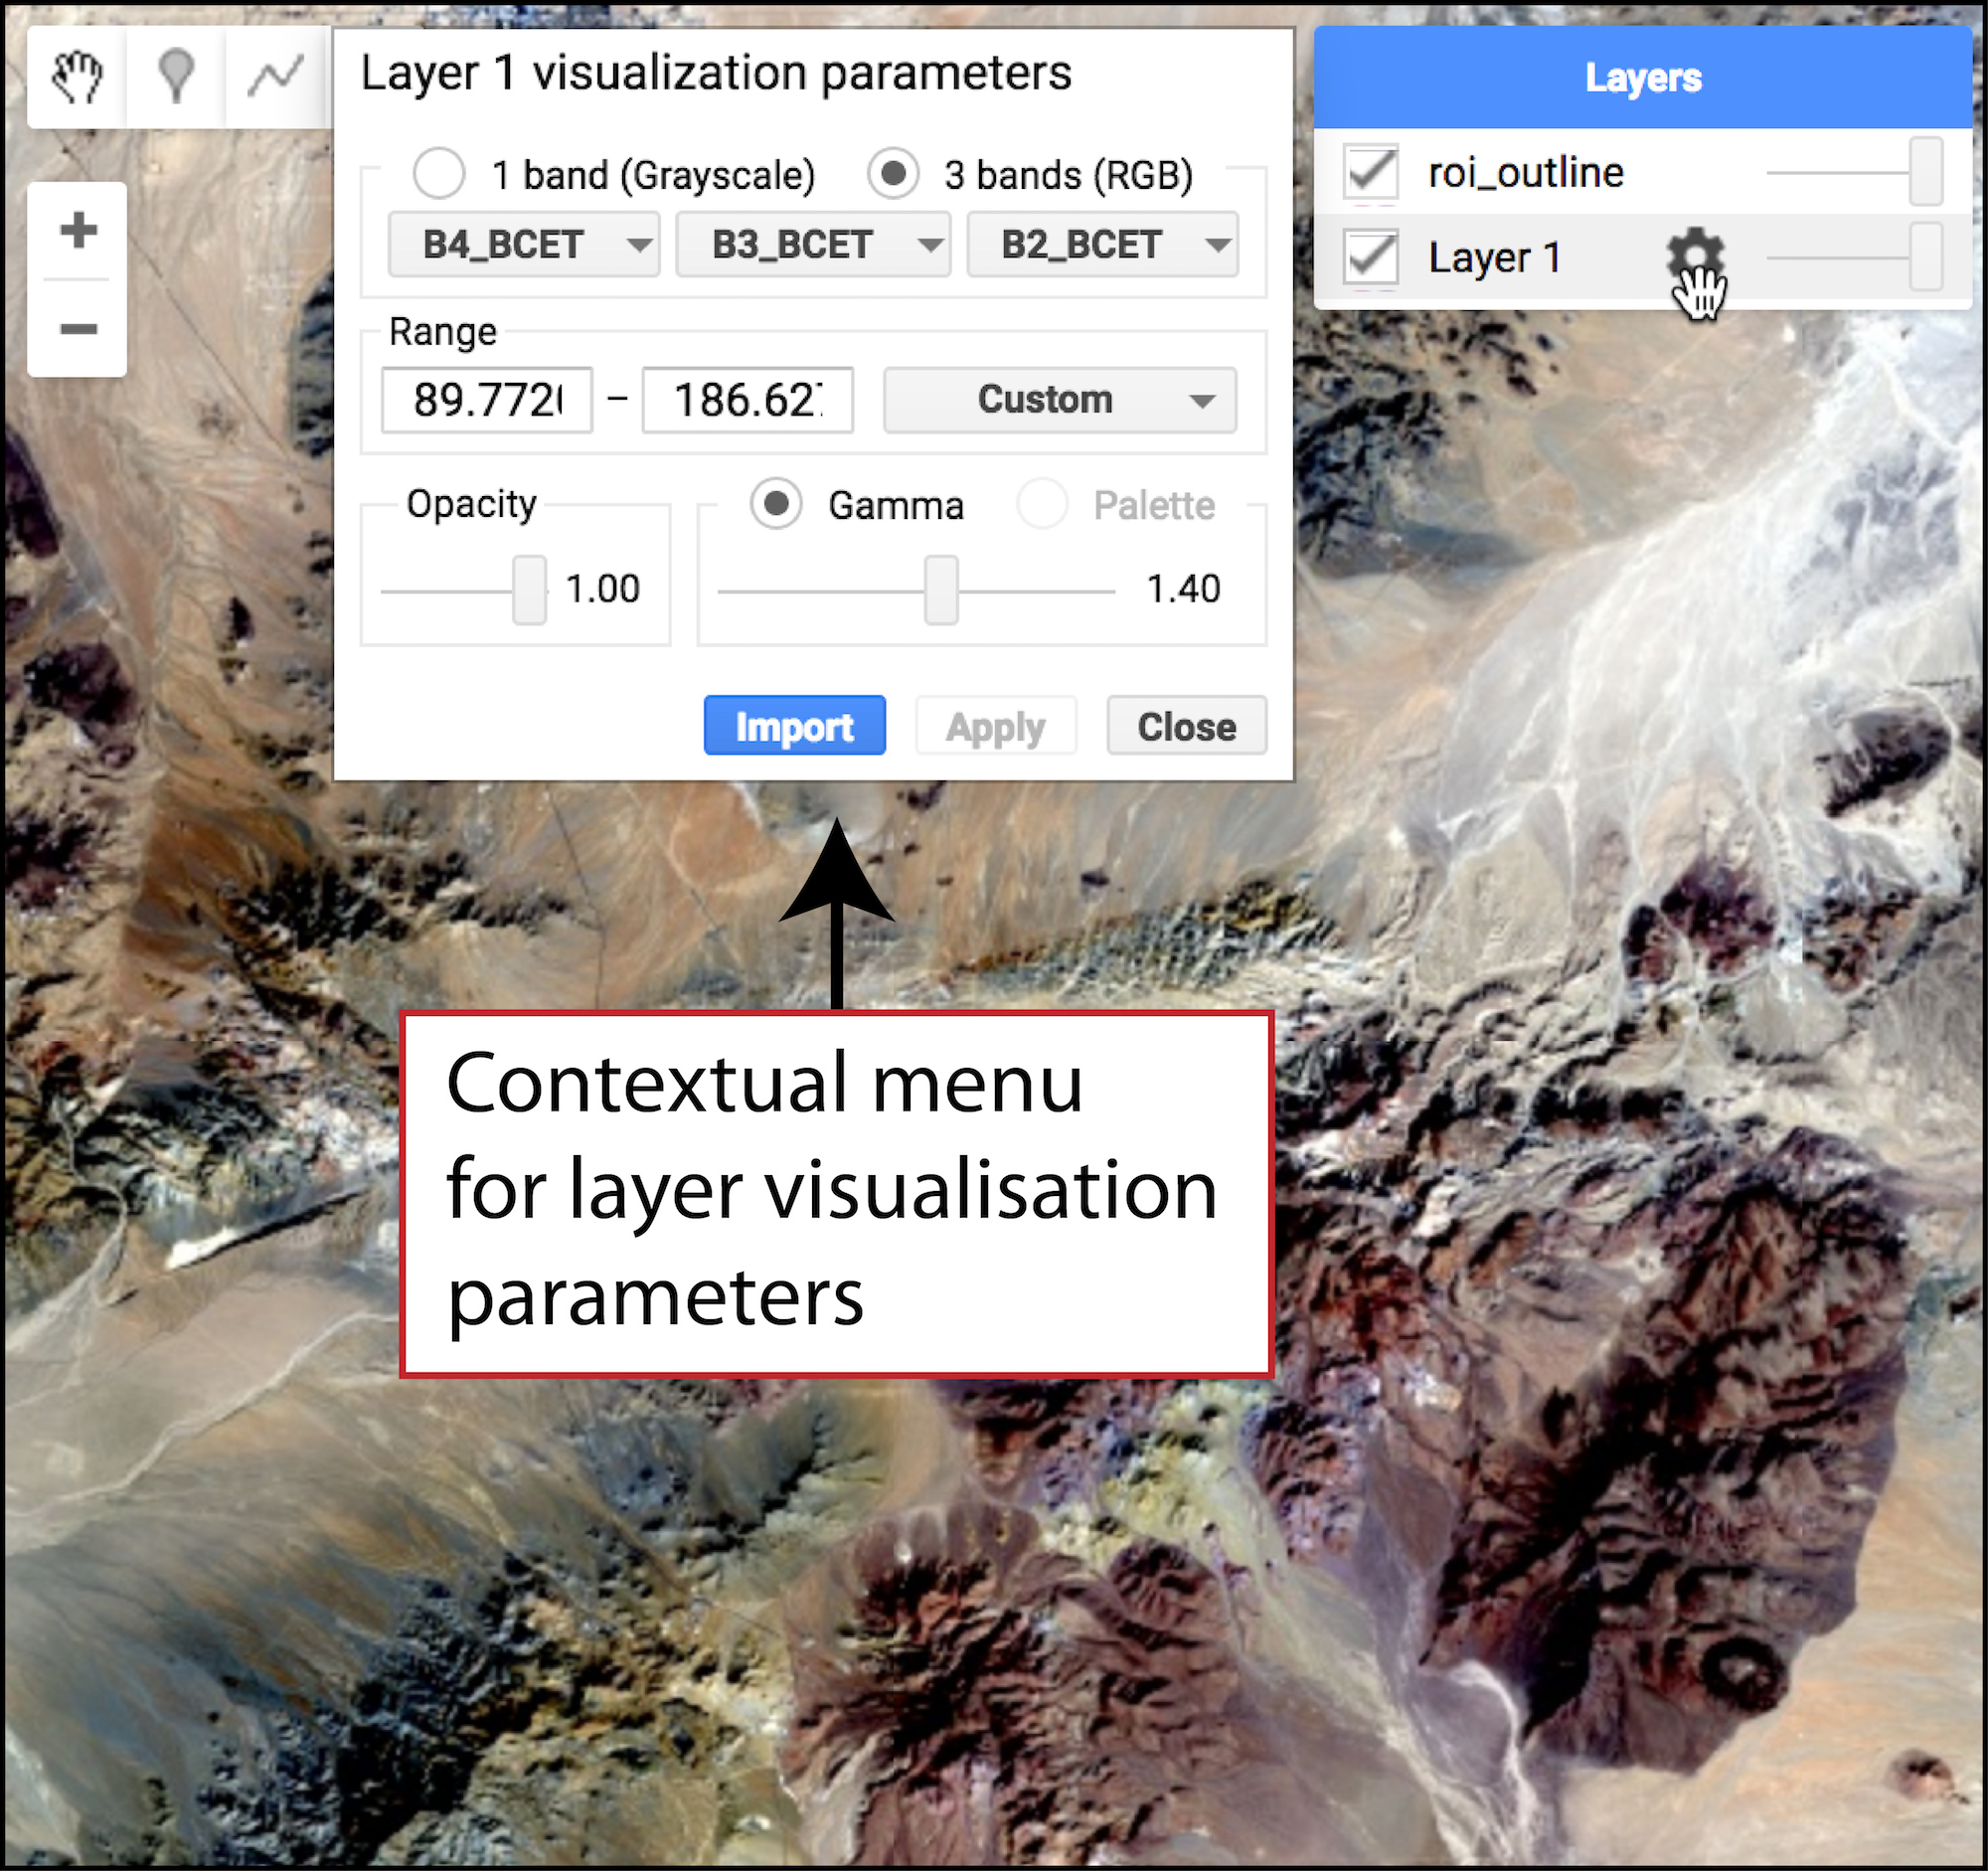
\includegraphics[width=0.5\textwidth]{images/layer_visualisation_reduced.jpg}
\caption{Example visualisation menu, accessible in the map viewport from the list of available layers.}
\label{fig:layer_visualisation}
\end{figure}

Figure~\ref{fig:choose_imagery}, details the selection of a Landsat 8 composite image to begin the ROI selection.

\begin{figure}[htbp]
\centering
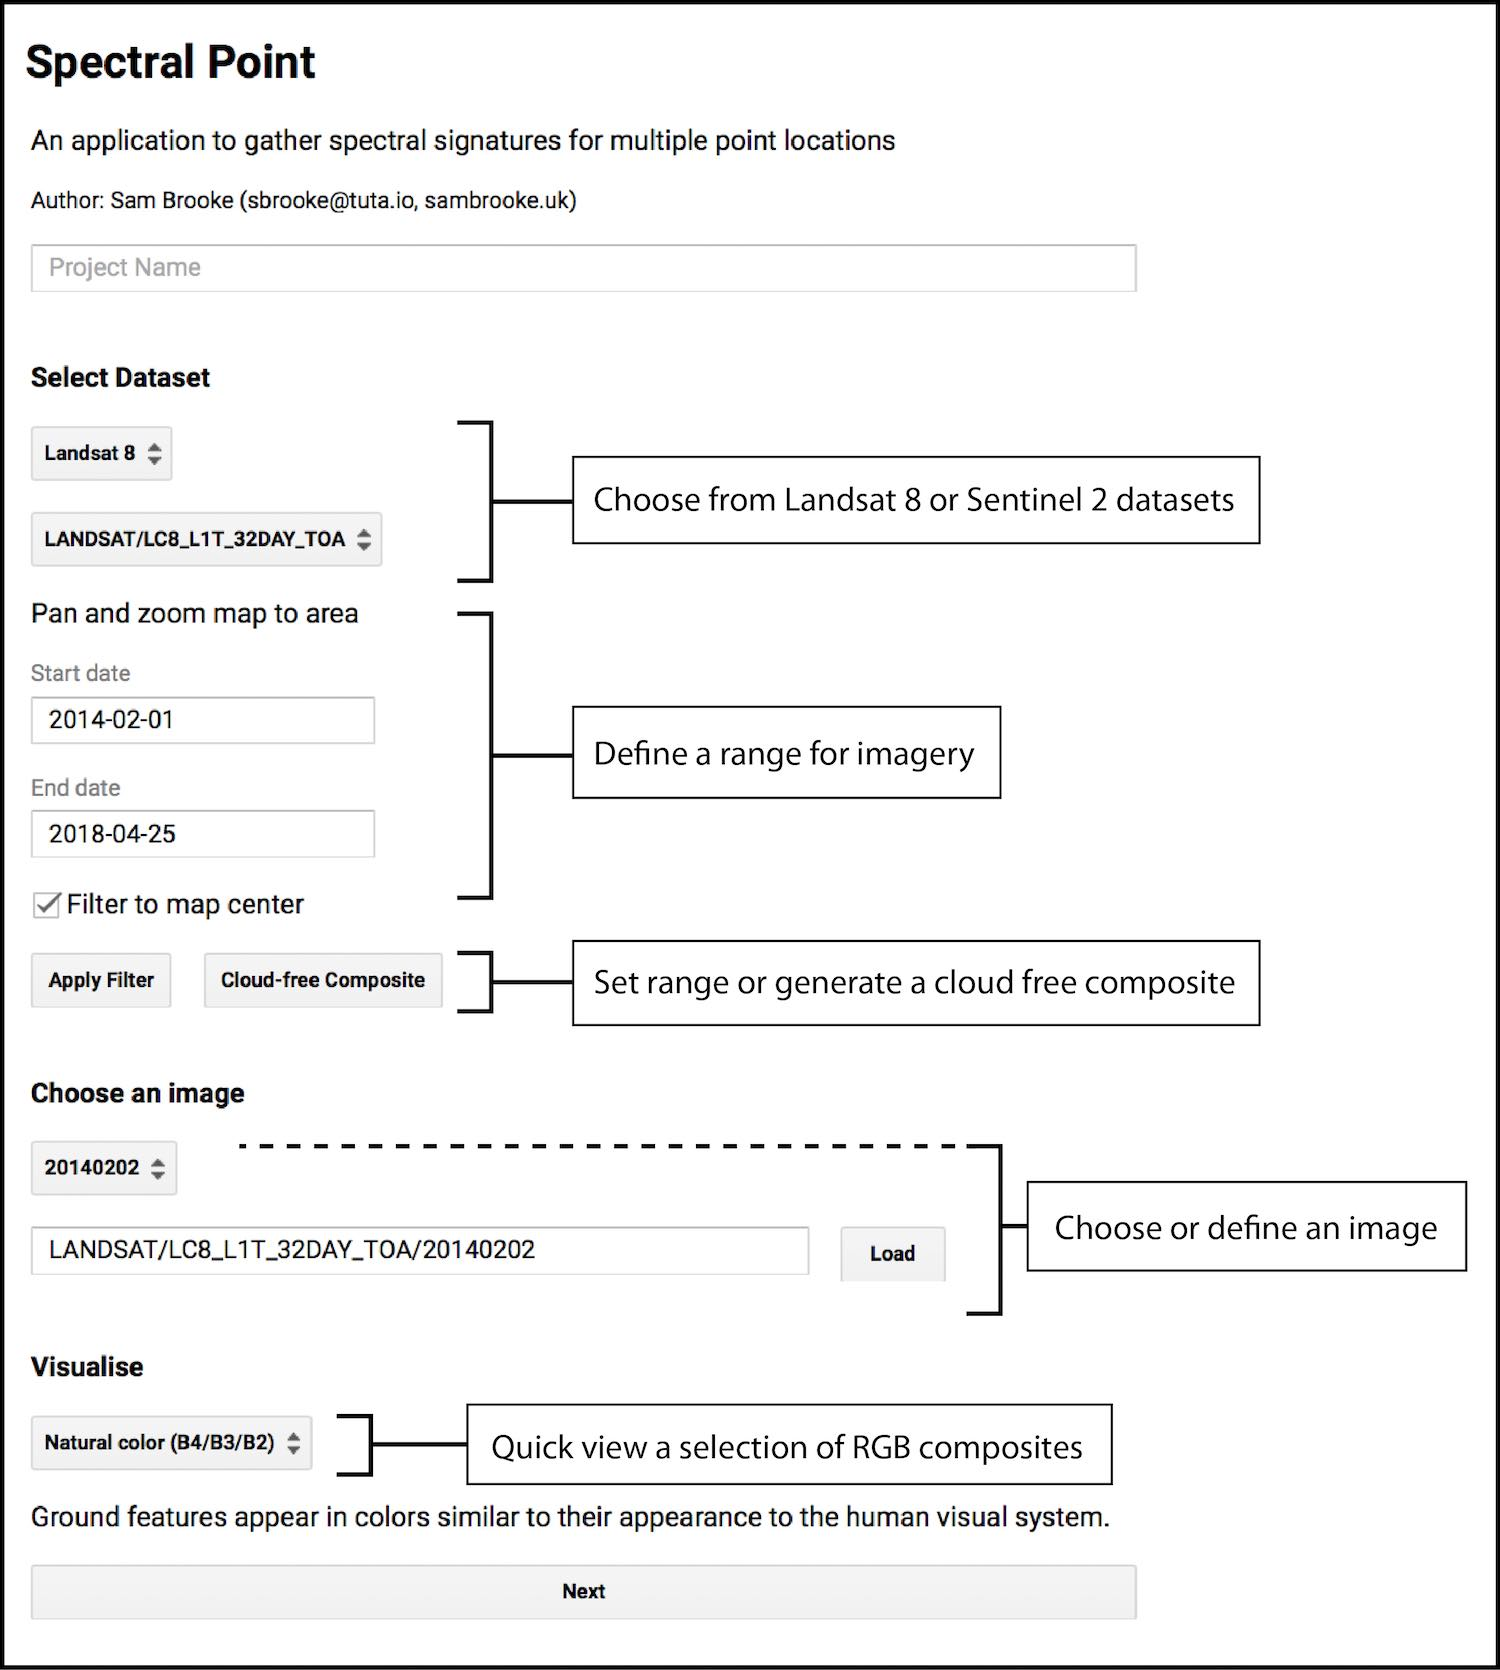
\includegraphics[width=0.8\textwidth]{images/choose_imagery_reduced.jpg}
\caption{The menu the user sees when first running the app is for the selection of a given Landsat 8 or Sentinel 2 aquisition, either as an 8 or 32 day composite stack. To help drill down to a given subset of images, a range of dates can be defined by the user, from which a drop down is populated, showing all available timestamps, or a cloud free composite generated if using Landsat data. In choosing an image, the mapping viewport will refresh to show the current Landsat composite, enabling the user to decide whether the imagery is suitable to their needs (i.e. isn't obscured by snow or cloud cover). A textbox is populated with the identifier of the give scene, which can be reloaded by simply copy-pasting when the application is run again. Once a scene is selected, a simple visualisation tool can change the default view from a basic range of RGB composites.}
\label{fig:choose_imagery}
\end{figure}

Once a suitable Landsat 8 scene has been selected click ``Next'' to proceed to the ROI selection menu.

\section{Defining a region of interest}

\fbox{\begin{minipage}{\textwidth}
\textbf{Note: } \textit{Spectral Point} may feel more unresponsive than a conventional desktop GIS application, especially when interacting with the map. This is to be expected as the input-output of given processes are negotiated with Google's servers and relayed back to the browser, so please be patient!
\end{minipage}}

\vspace{2em}

\textit{Spectral Point} requires that the user define a region of interest or ROI for further image processing, specifically contrast enhancement (See section~\ref{sec:BCET}) and principal component analysis (See section ~\ref{sec:vis_and_pca}). The application will not continue until an ROI is set. The ROI should be an area that encompasses at least the intended study area, but will inevitably encumber the application's performance or exceed GEE memory limits if the area is too large. The menu for ROI selection is outlined in figure~\ref{fig:ROI_menu}, with a step-by-step diagram in figure~\ref{fig:roi_steps}. It is imporant to note that \textit{Spectral Point} utilises the ``best effort'' approach to image computation, which recomputes the scale of any raster processing in order to not exceed the maximum value of 10 million pixels allowed by GEE.

\begin{figure}[htbp]
\centering
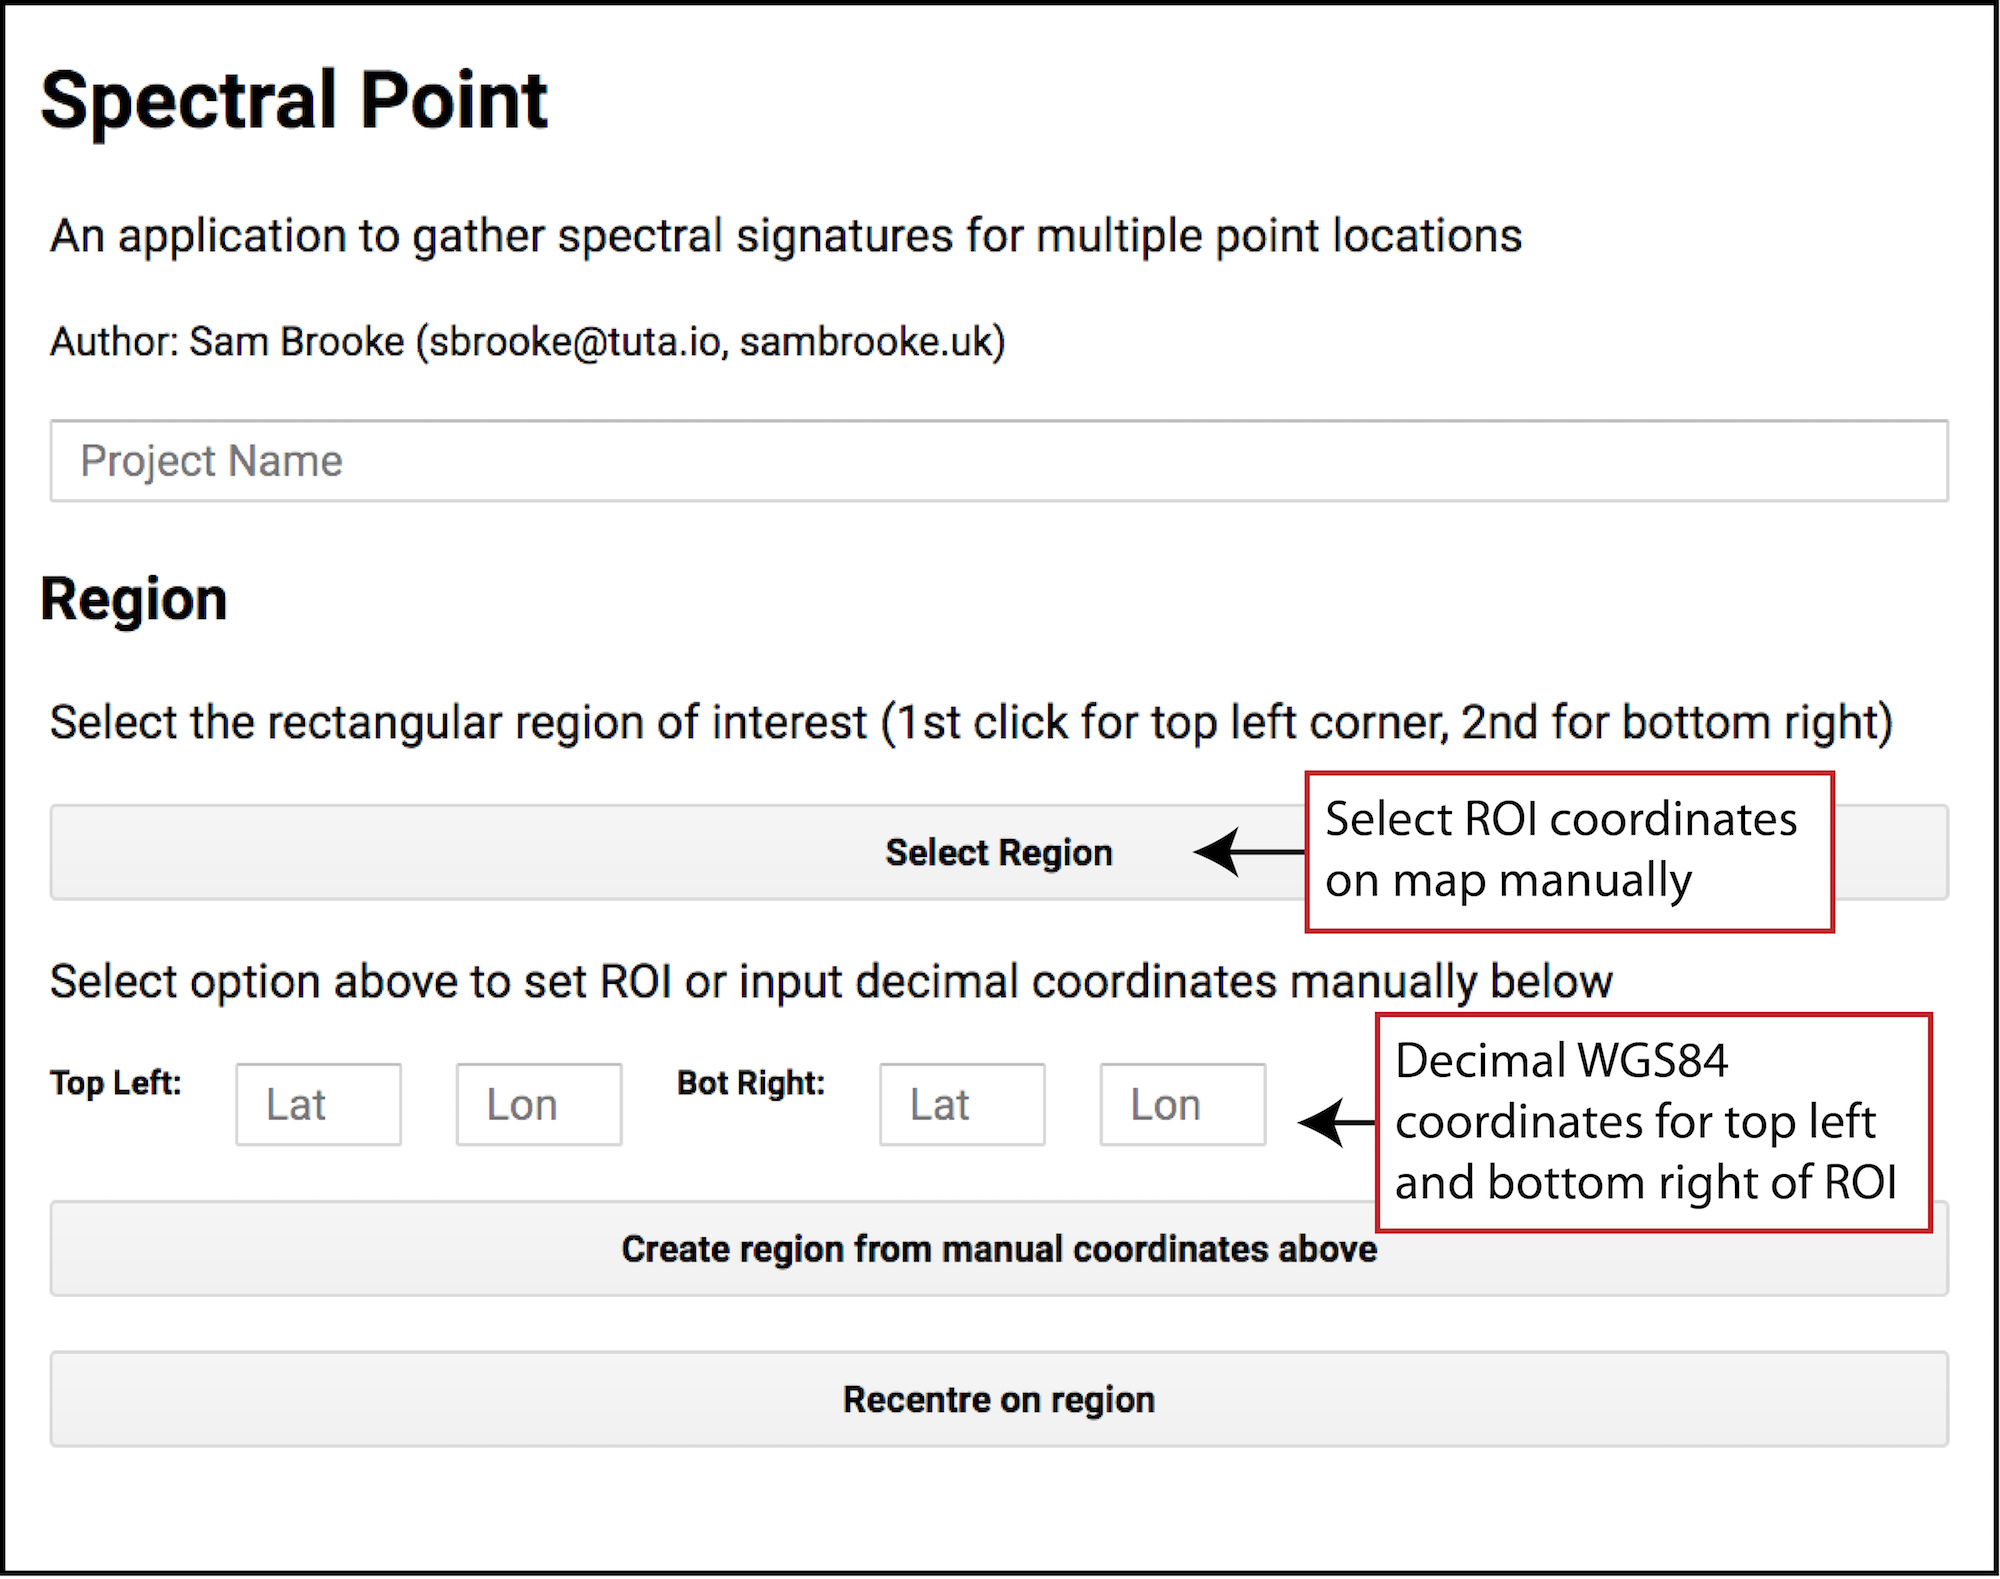
\includegraphics[width=0.7\textwidth]{images/ROI_menu_reduced.jpg}
\caption{The second menu provides two options to generate a region of interest or ROI, that should encompass at least the extent of the user's study area. This first method to generate an ROI requires the user to click ``Select region'' and click twice on the map to produce a rectangular region outline, once for the top left of the rectangle and the second click for the bottom right extent of the rectange (See Figure~\ref{fig:roi_steps}). After an ROI has been created, the four text boxes will populate with the decimal coordinates of the ROI top-left and bottom-right extents. These text boxes also enable the user to generate an ROI by inputting these decimal coordinates manuall and clicking the button below.}
\label{fig:ROI_menu}
\end{figure}

\begin{figure}[htbp]
\centering
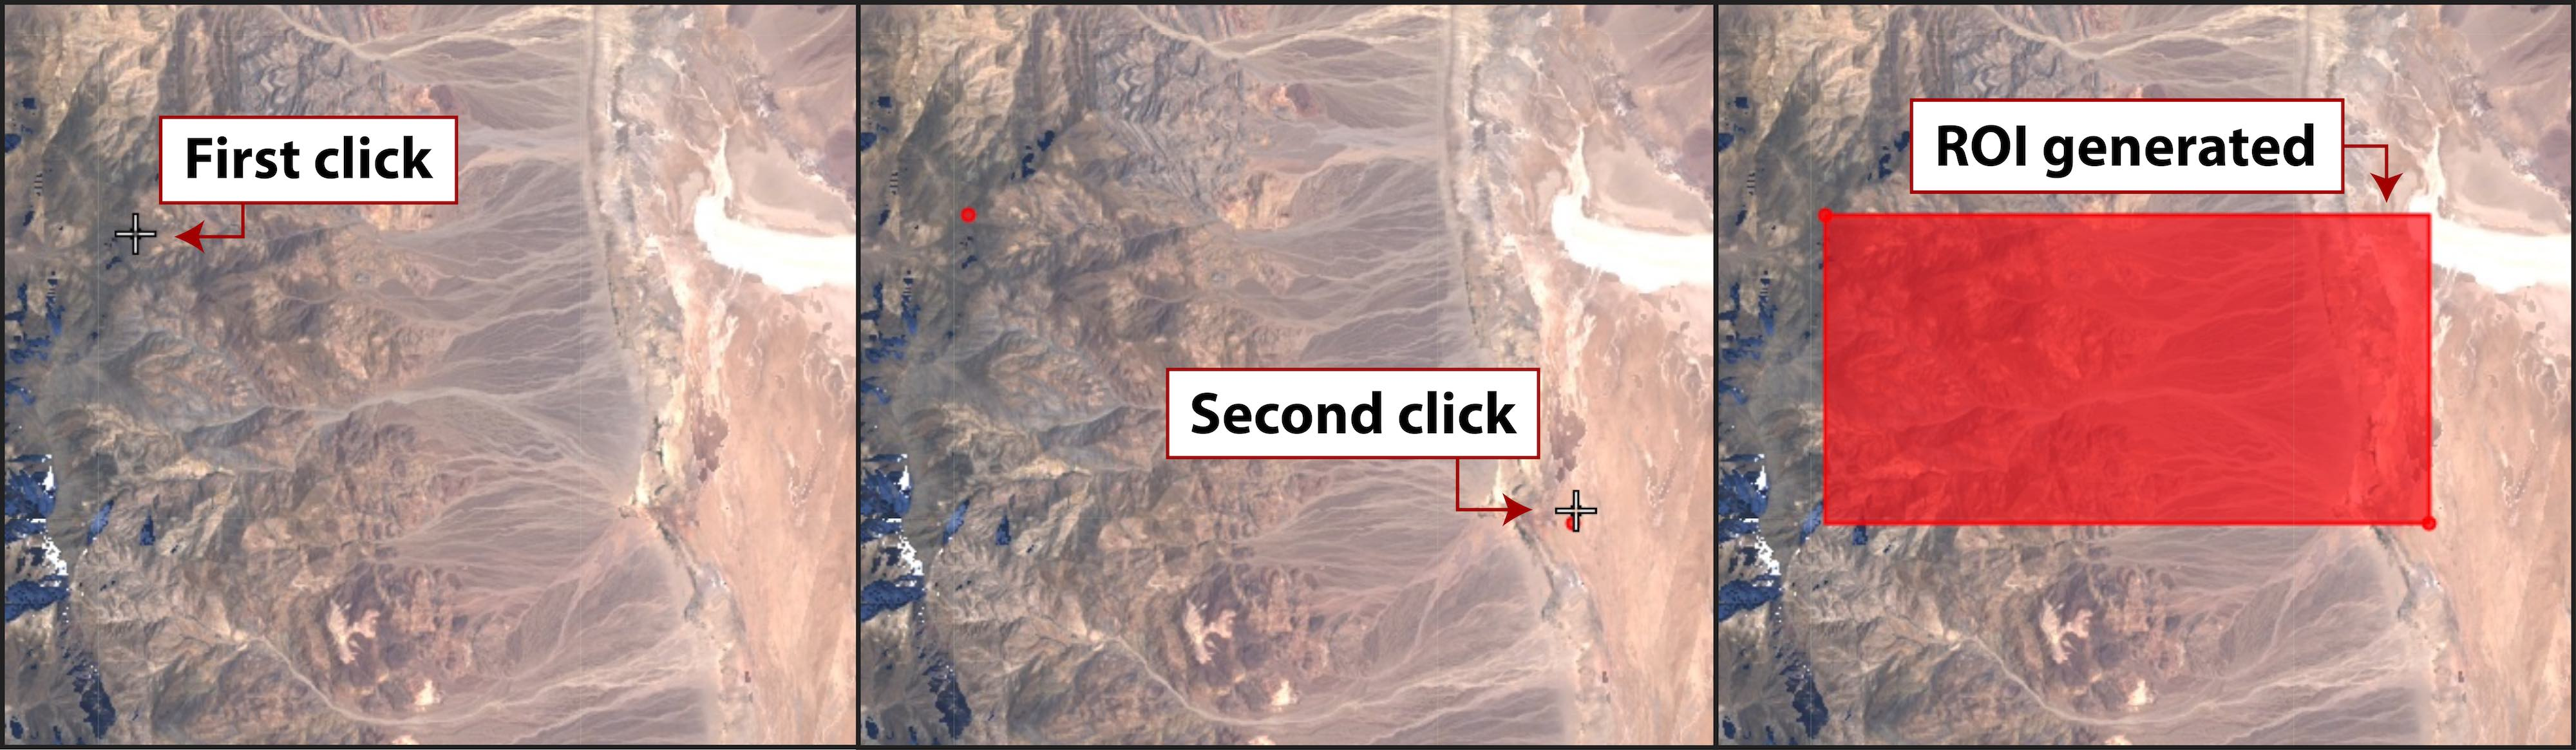
\includegraphics[width=1.0\textwidth]{images/roi_steps_reduced.jpg}
\caption{Step-by-step ROI generation using manual two-click method (See figure~\ref{fig:ROI_menu})}
\label{fig:roi_steps}
\end{figure}


\section{Contrast enhancement}
\label{sec:BCET}

Once an ROI has been set, the next menu will provide the option to normalise the spectral bands, useful for improving the visual quality of images as well as band cross-comparison \citep{guo1991,LiuMason2009}. An example of the BCET algorithm applied to different spectral bands can be seen in figure~\ref{fig:histograms}. The option to perform contrast enhancement is labelled ``BCET Region'', but a user can skip this step to investigate an unmodified Landsat 8 composite.

\begin{figure}[htbp]
\centering
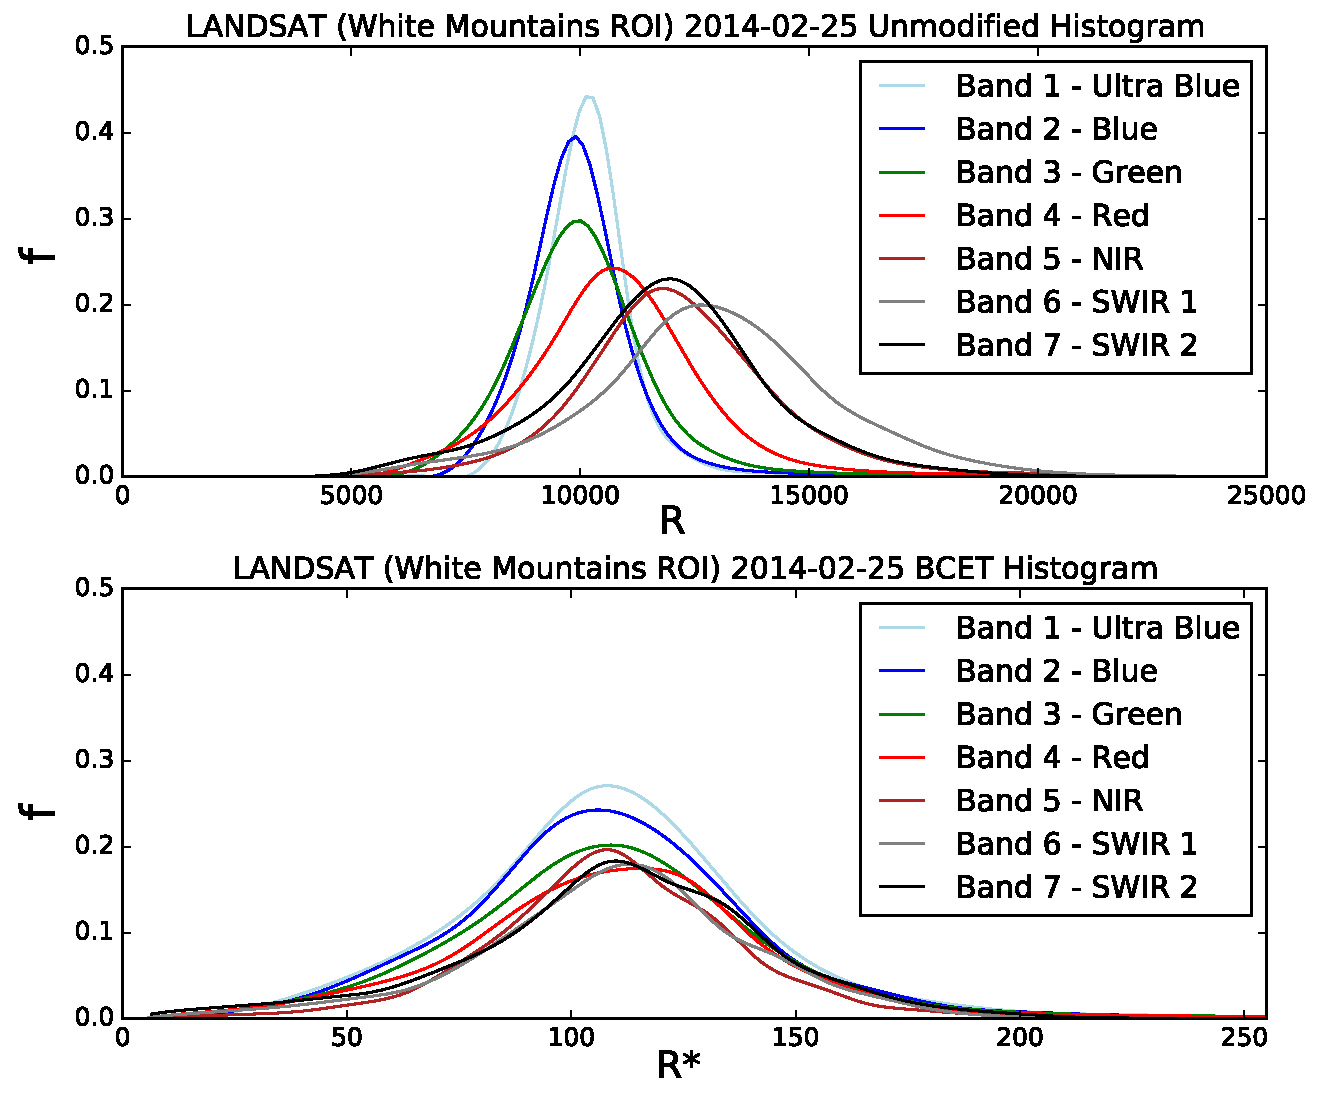
\includegraphics[width=1.0\textwidth]{images/histograms.pdf}
\caption{Reflectance value histograms for each Landsat 8 band in the visible to the short-wave infrared (SWIR). Top: Reflectance histograms for unmodified Landsat 8 TOA image bands. Bottom: Histograms for Landsat 8 TOA image bands have been normalised using the balance contrast enhanced technique or BCET \citep{guo1991}, each with a minimum R* value of 0, a maximum of 255 and mean of 110.}
\label{fig:histograms}
\end{figure}

In general, BCET (balance contrast enhancement technique, \citet{guo1991,LiuMason2009}) is an effective method to eliminate colour bias in the image and to enhance the spectral contrast between bands. \textit{Spectral Point} uses BCET to normalise the histograms from bands 1-7 (Ultra blue to short wave infrared) and the thermal infrared bands 10 and 11 \citep{barsi2014}. Once implemented, the BCET algorithm is applied to the entire viewable portion of Landsat images based on the image statistics of the ROI.

\section{Visualisation and PCA}
\label{sec:vis_and_pca}

The next menu, shown by figure~\ref{fig:pca}, provides the option for performing principal component analysis (PCA) on and subset of multispectral bands. This option is not required to continue, but can be an effective tool to investigate patterns and variation between multispectral bands.

The mapping viewport can be changed to any combination of bands in an RGB composite by selecting them in the three drop down lists within the layer contextual menu (See Figure~\ref{fig:layer_visualisation}). This band should be a useful visualisation for the given study, but can be altered and adjusted at any time either by viewing either the ``All Bands'' or ``BCET Bands'' layer, depending on whether contrast enhancement has been performed (See Figure~\ref{fig:available_bands}).

\vspace{2em}
\begin{figure}[htbp]
\centering
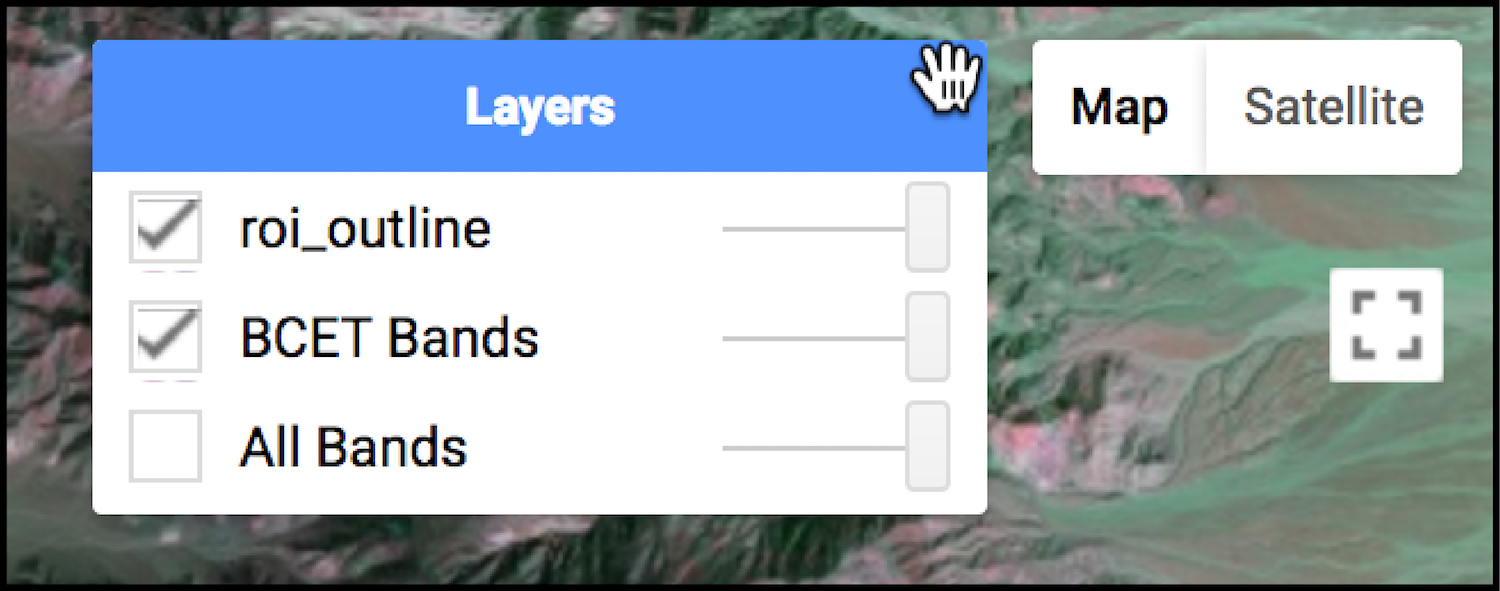
\includegraphics[width=0.5\textwidth]{images/available_layers_reduced.jpg}
\caption{The bands available to manipulate in the layer dropdown after BCET normalisation. If BCET has not been performed only the ``All Bands'' layer will be visible.}
\label{fig:available_bands}
\end{figure}


\begin{figure}[htbp]
\centering
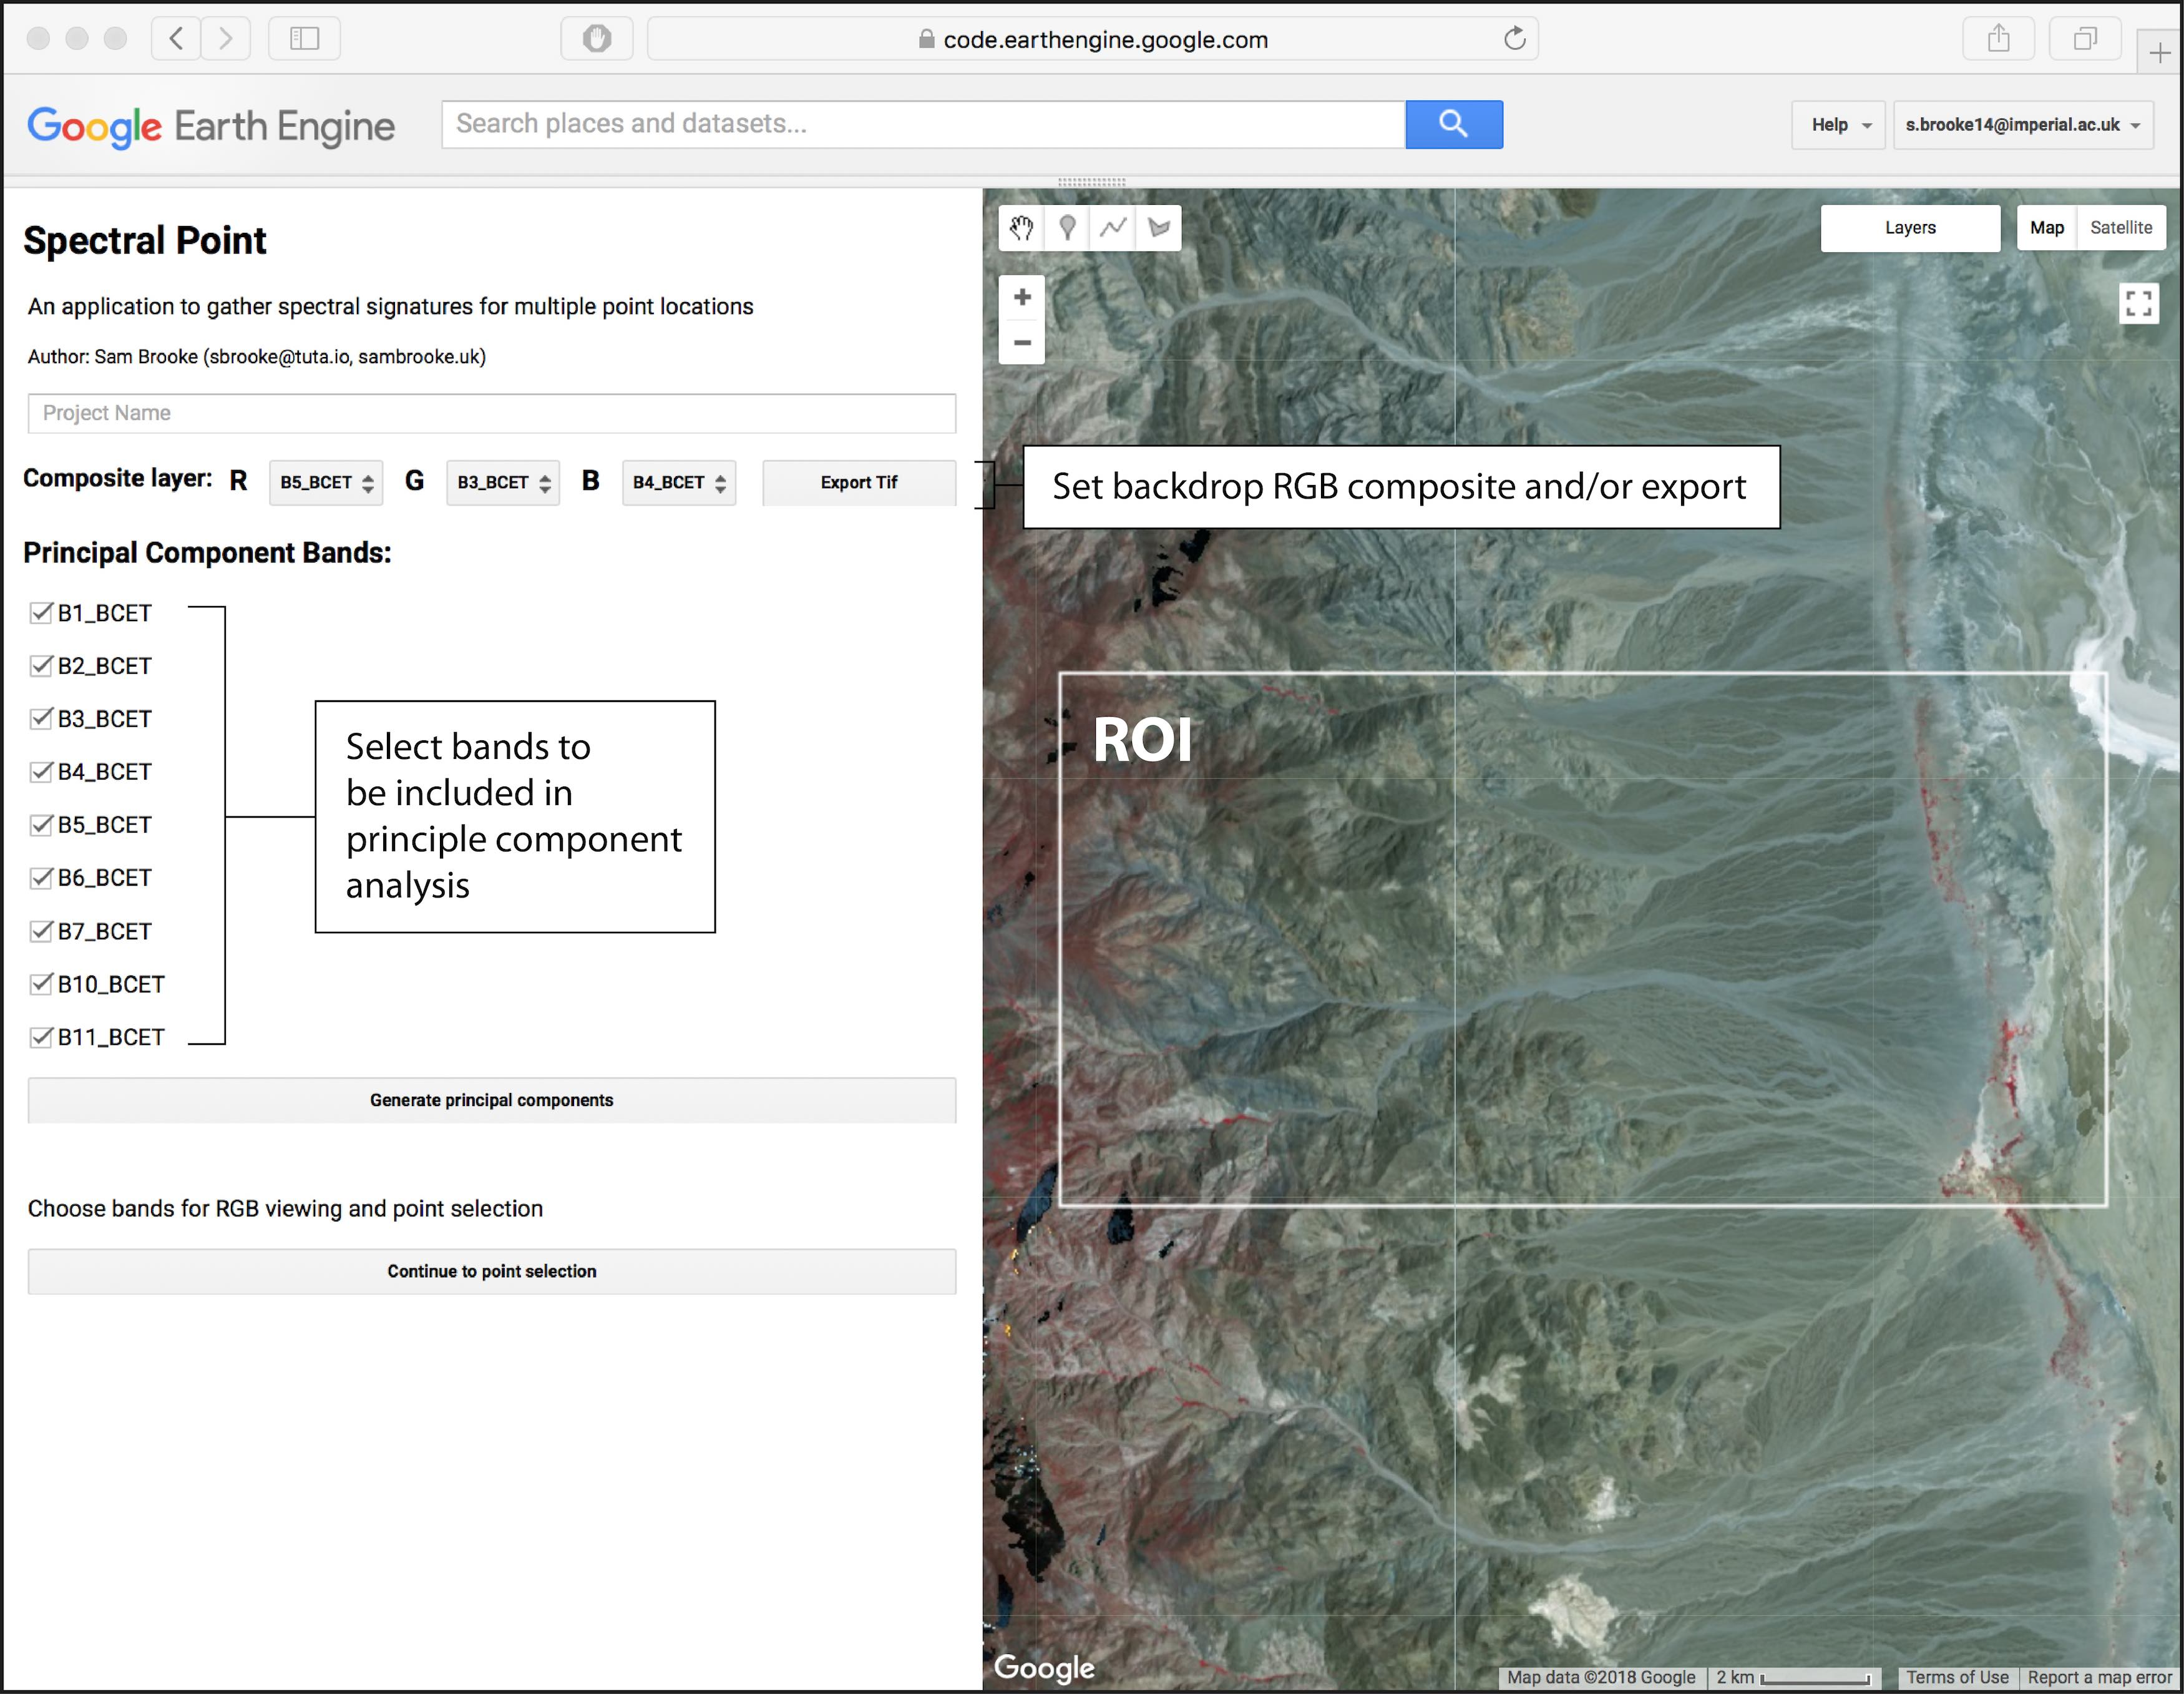
\includegraphics[width=1.0\textwidth]{images/pca_reduced.jpg}
\caption{This menu follows the choice to either perform BCET processing on the Landsat 8 image or to skip. This menu is intended to provide the user a further means to generate an RGB image of any combination of bands in the Landsat 8 composite, both for export as a geotiff or as background imagery during final spectral point collection. The list of bands available principal component analysis (PCA) will be suffixed with ``\_BCET'' if the bands have been normalised. PCA is only processed if the user selects ``Generate principal components''.}
\label{fig:pca}
\end{figure}

\section{Selecting Points}
\label{sec:selecting_points}

With the chosen RGB visualisation of Landsat imagery, \textit{Spectral Point} enables the user to select a range of query points either by either interactive selection on the image, single coordinate input or the loading of a premade set of coordinates from Google's Fusion Table data visualisation/storage service. Each option will load a series of points into the menu that can subsequently be removed or selected to reorient the viewport to the query point’s location. Depending on which bands the user chooses to collect data from, a band reflectance chart is displayed and automatically updated with each additional point selection. As seen on the screenshot in Figure 2, a user can immediately view the spectral profile of any point within the map viewport and compare any selection of points across a range of spectral bands. As a visual aid, the user can also produce a semi-transparent Kirsch-filtered edge detection layer to highlight areas that may be subject to edge or boundary effects.

\subsection{Selecting RGB bands}

\begin{figure}[htbp]
\centering
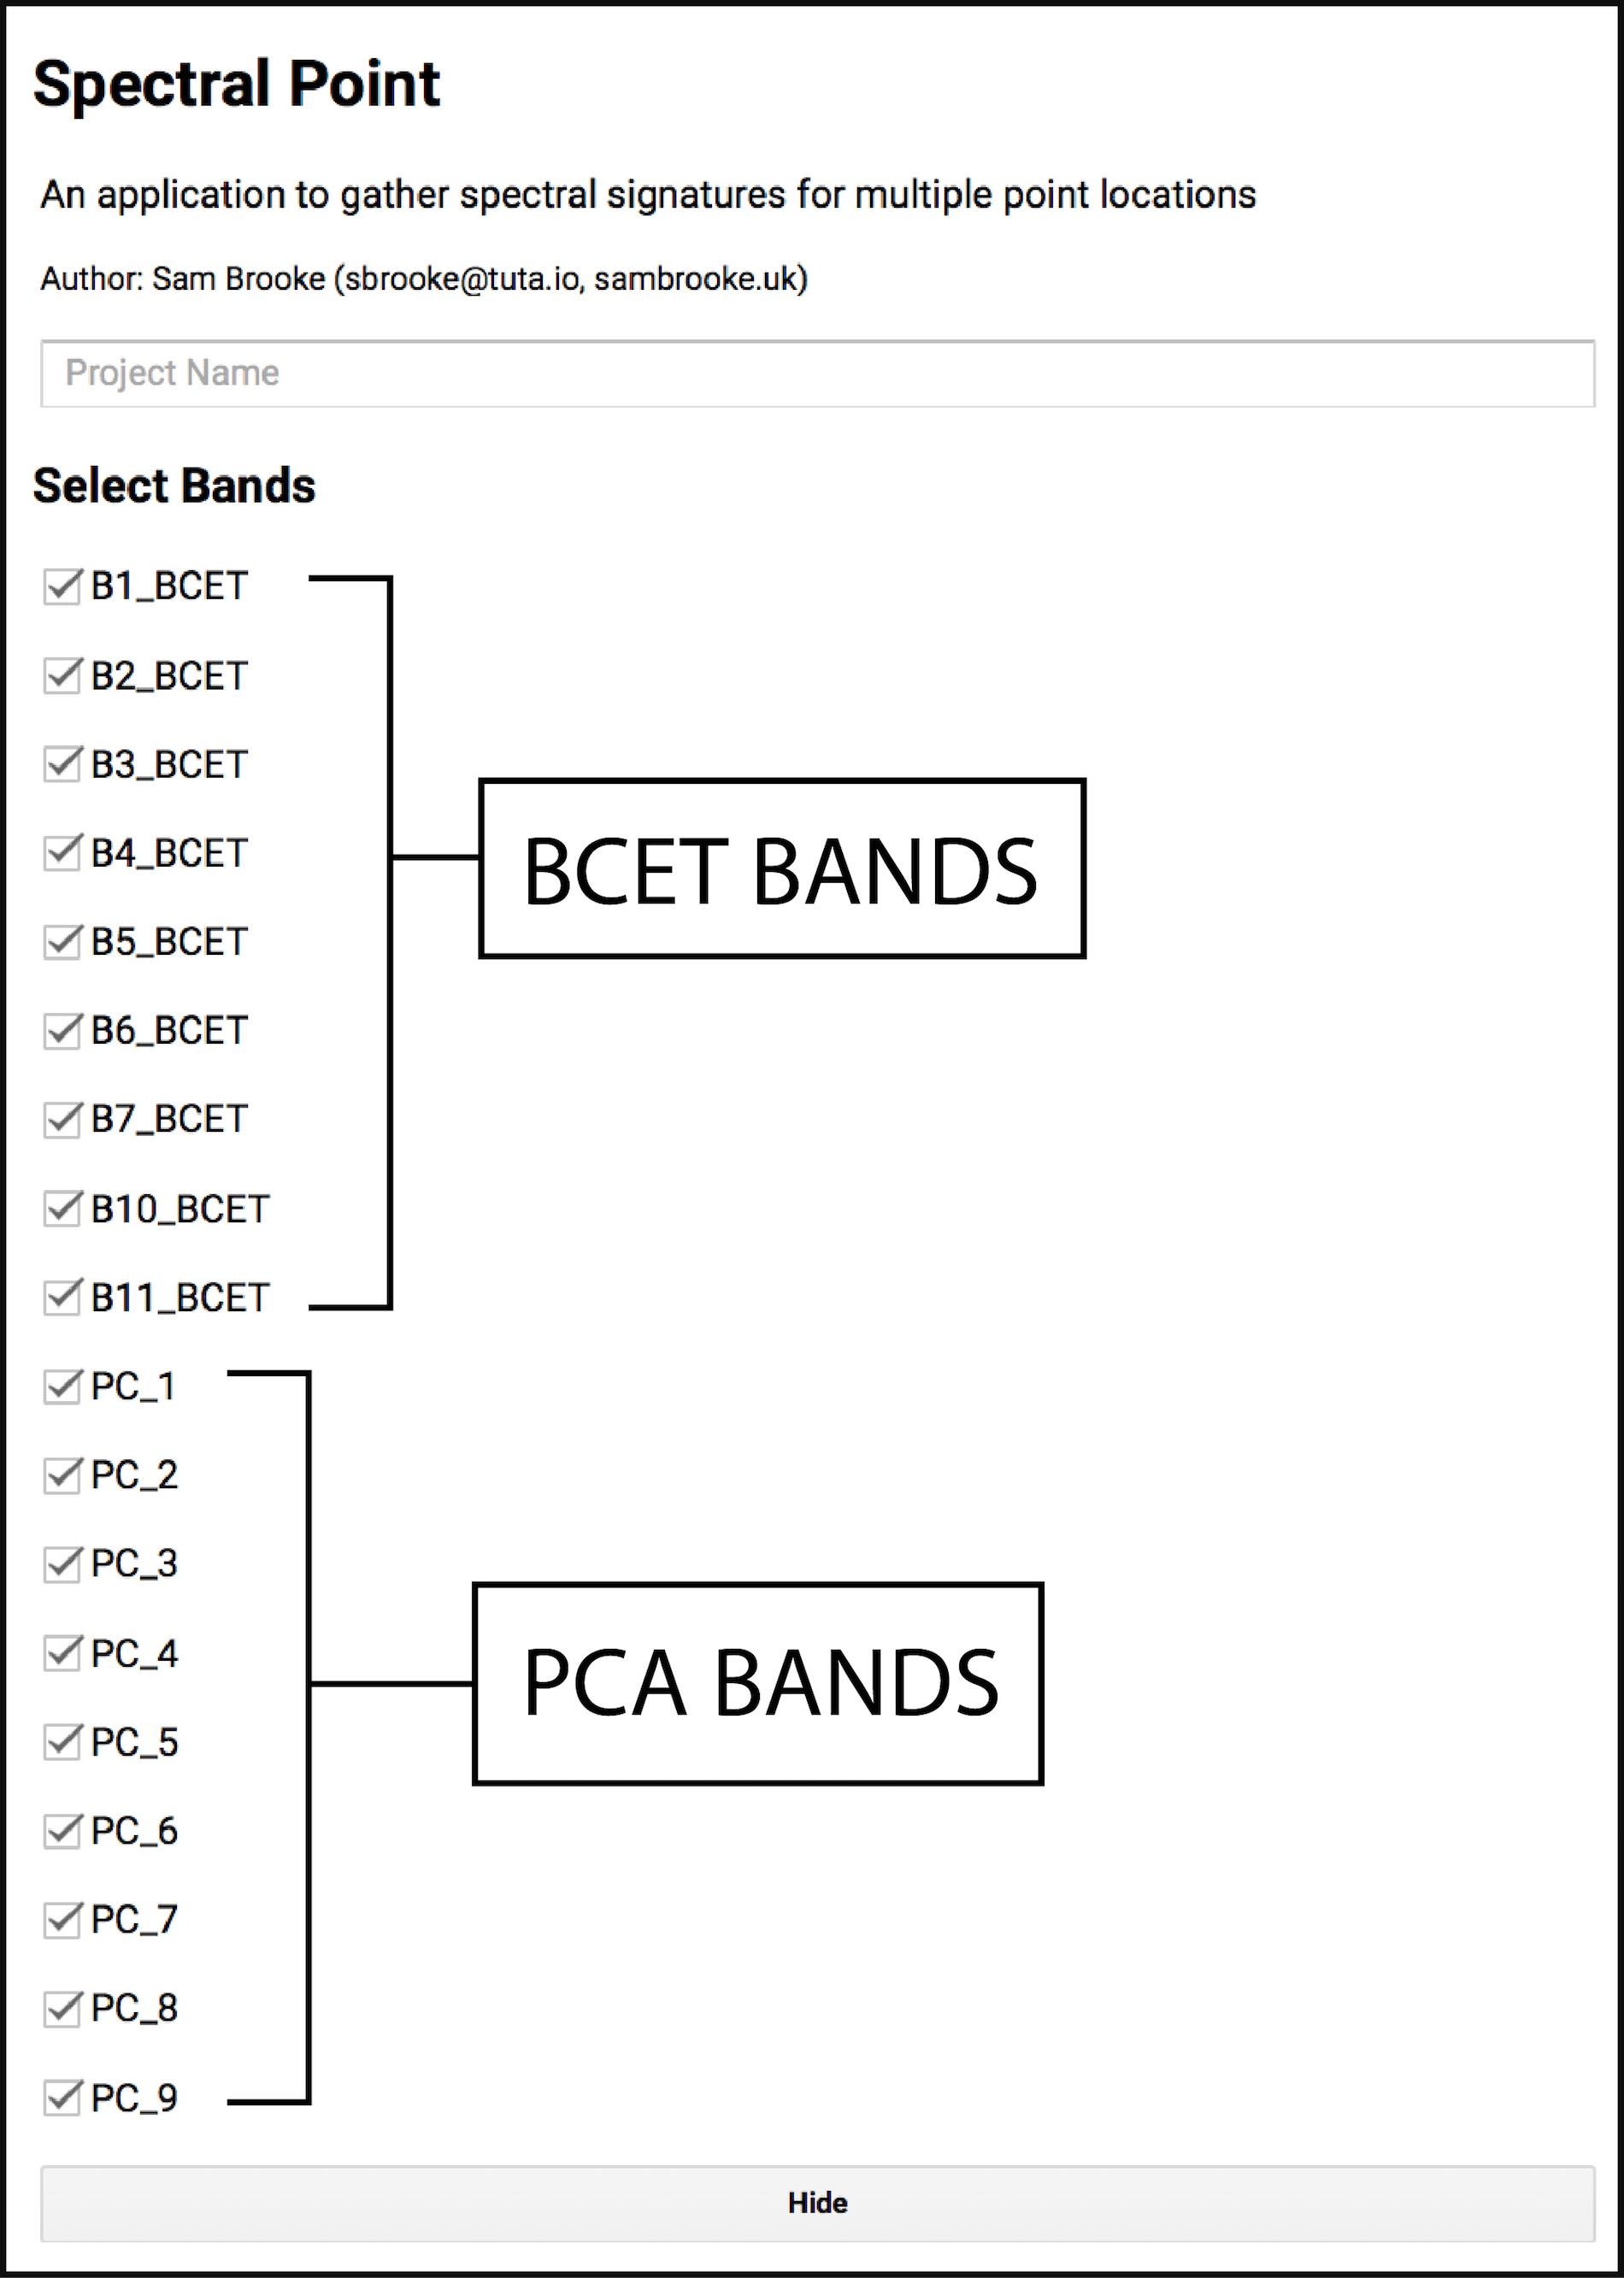
\includegraphics[width=.5\textwidth]{images/choose_bands_reduced.jpg}
\caption{The choice of bands shown is a list of all bands available after BCET or PCA processing. The list does not determine the range of bands used when exporting data (See section~\ref{sec:export-data}), but only the bands plotted in the preview chart (See figure~\ref{fig:select_points}).}
\label{fig:choose_bands}
\end{figure}

\subsection{Manual Selection}

Figure~\ref{fig:select_points} shows the point selection interface, with an example set of points collected on the Hanaupah Canyon fan, Death Valley, California. These points correspond by colour to the list of points in visible in the top left of the figure, which can be removed or used to recentre the map viewport. To begin creating points, a user must select ``Select points on map'' to begin click on locations within the map view extent. ``Pan mode'' will return the cursor to the default mode without selecting points unintentionally on each click. The preview chart of pixel values will auto update after each point is added or removed. Predefined points can be added using the text box inputs, with a user-defined sample name, and WGS84 latitude and longitude.

\vspace{2em}
\fbox{\begin{minipage}{\textwidth}
\textbf{Note: } Given that pixel locations can intersect ambiguously with edges in the Landsat image, a Kirsch edge detection filter can also be added to the map to act as a visual aid to select areas with less edge interference.
\end{minipage}}

\begin{figure}[htbp]
\centering
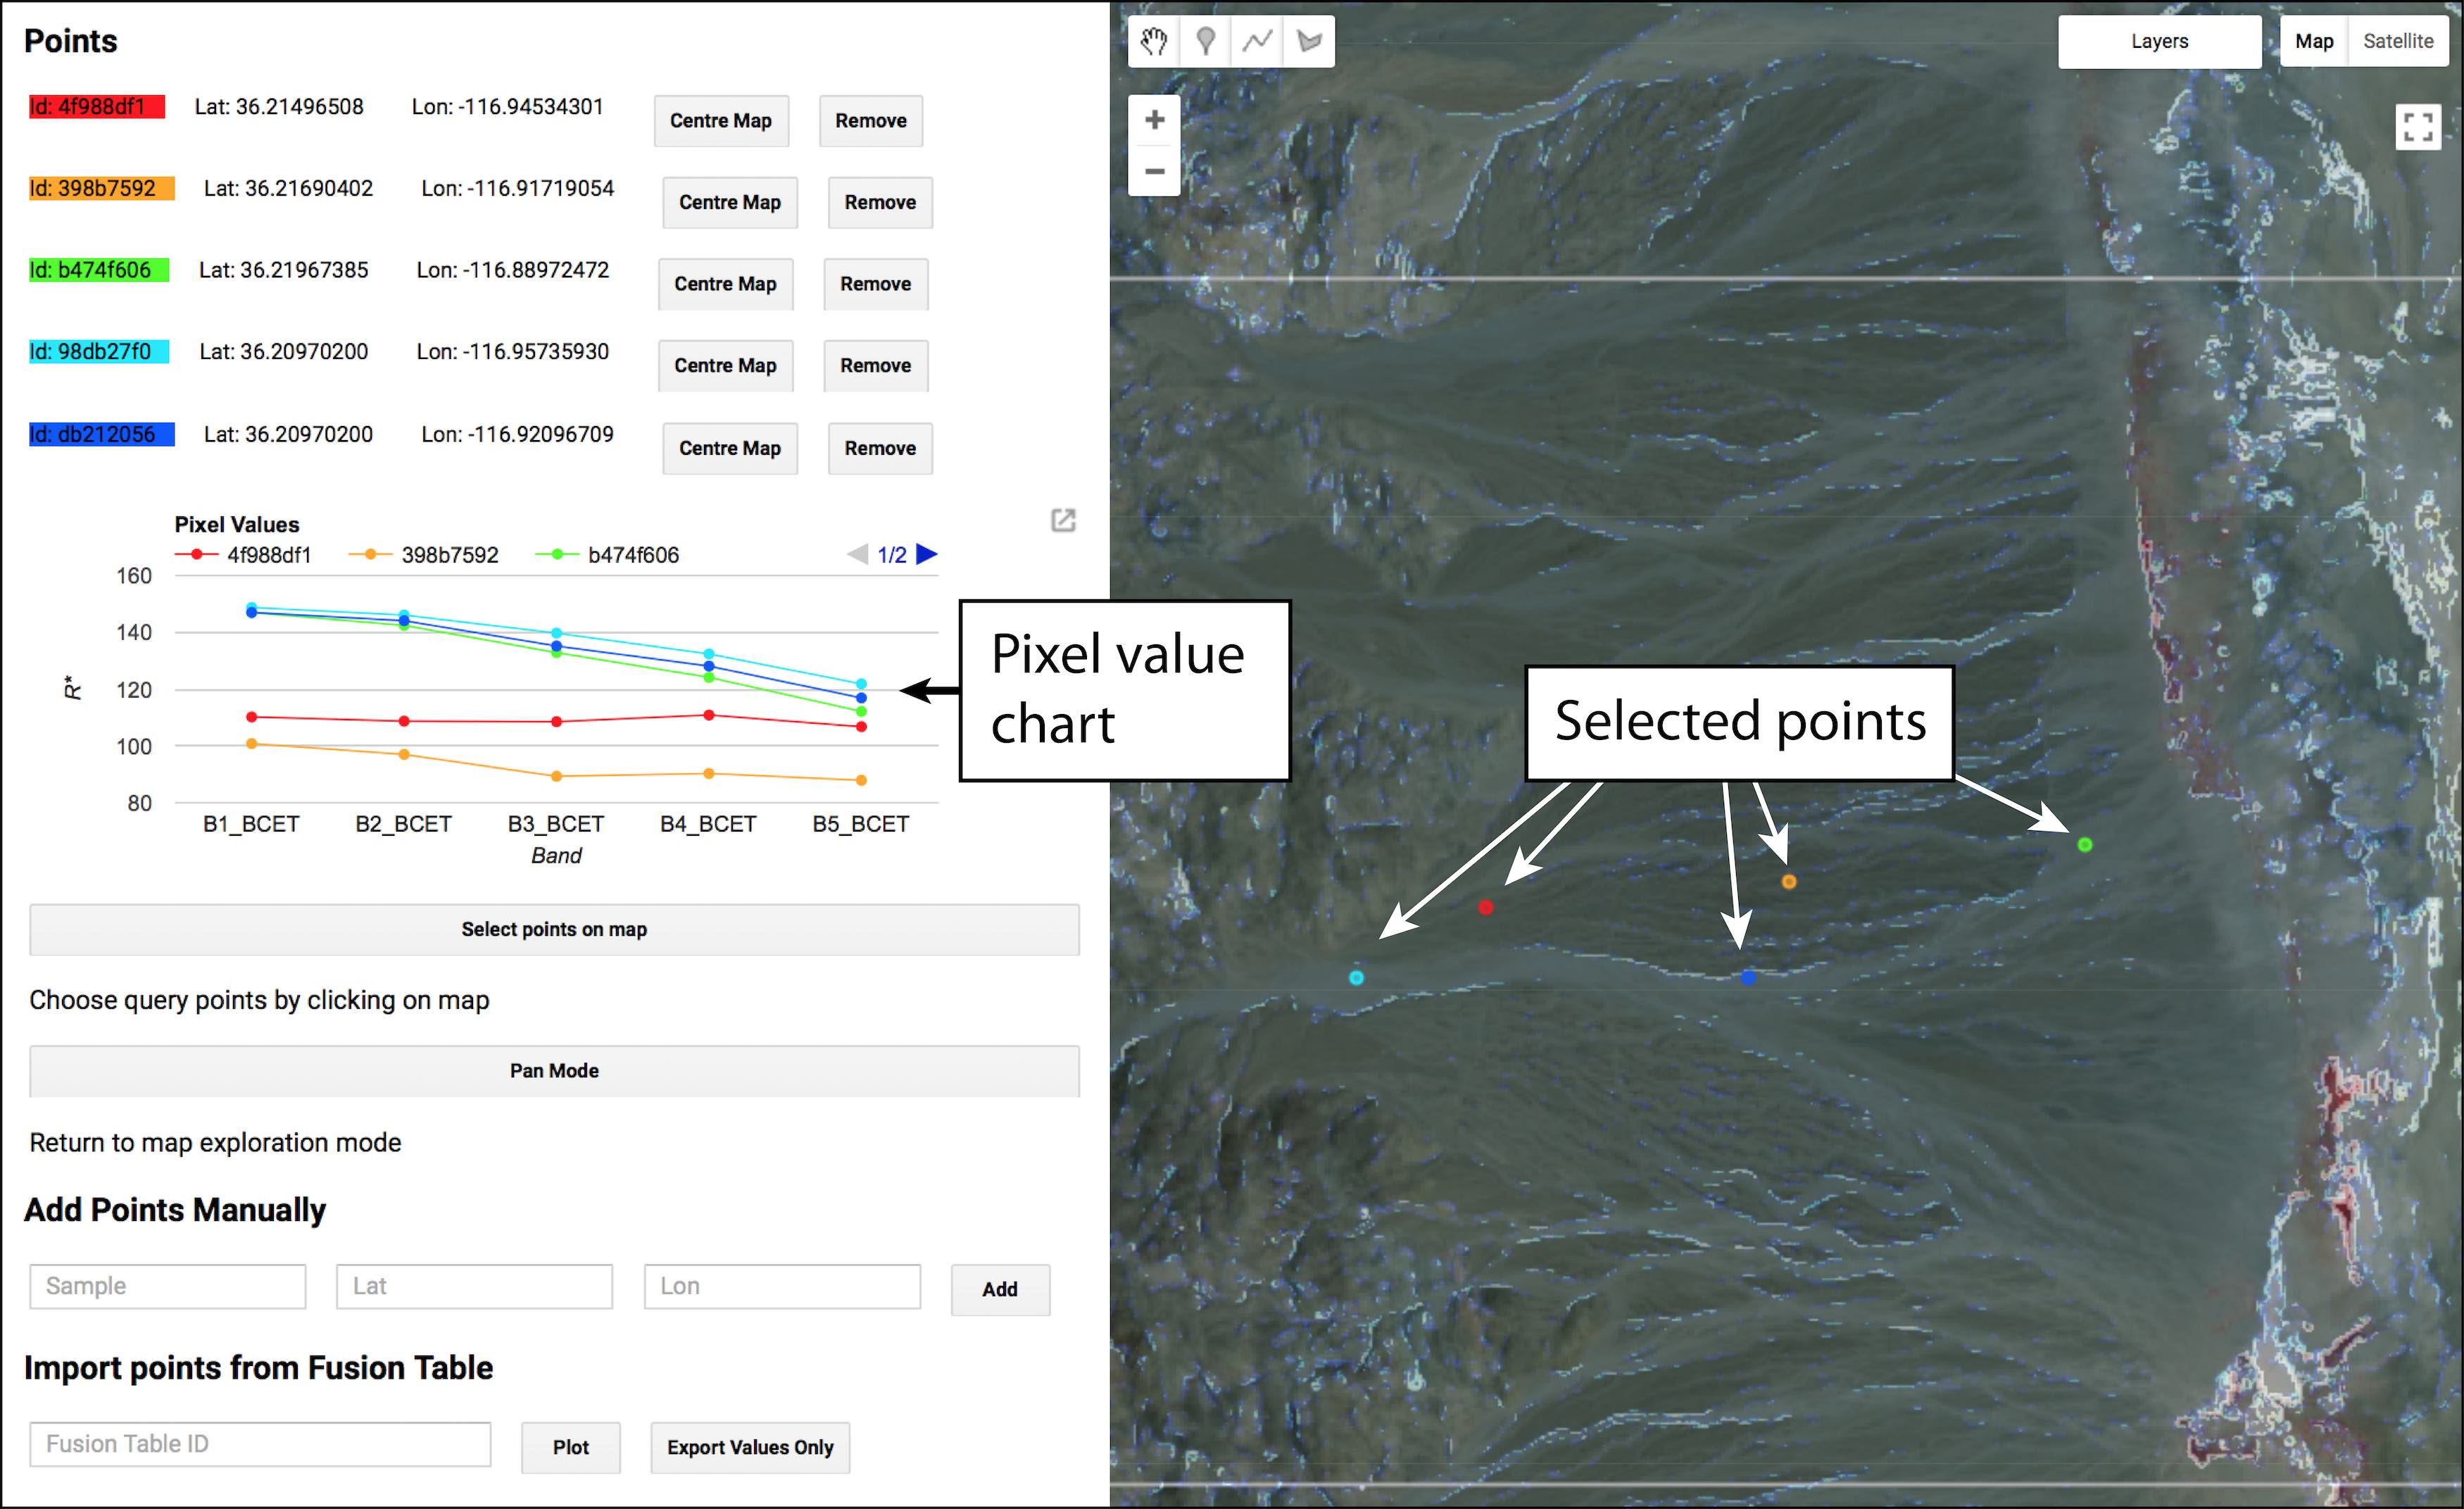
\includegraphics[width=1.0\textwidth]{images/select_points_reduced.jpg}
\caption{\textit{Spectral Point} screenshot showing the application layout within the GEE environment. The left third of the image contains the custom user interface menu during the spectral point selection stage, with options to add an edge detection layer, view spectral information of a series of query points, input new coordinates and export data. The right two thirds of the screenshot contain the image viewport with the current multispectral RGB composite displayed with an edge detection overlay. The multi-coloured points on the image mark the locations of current query points, which correspond in terms of marker and line colour to the list of points on the left menu and the individual lines of the pixel value chart. The pixel value chart can be exported as an image and csv file by itself.}
\label{fig:select_points}
\end{figure}

\subsection{Loading from fusion table}
\label{sec:fusion_table}

For a multitude of predefined query points \textit{Spectral Point} utilised GEE's interface with Google's Fusion Table format (\href{https://fusiontables.google.com}{fusiontables.google.com}). The workflow for adding fusion table data is illustrated in figure~\ref{fig:fusion_table}.

\begin{landscape}
\begin{figure}
\centering
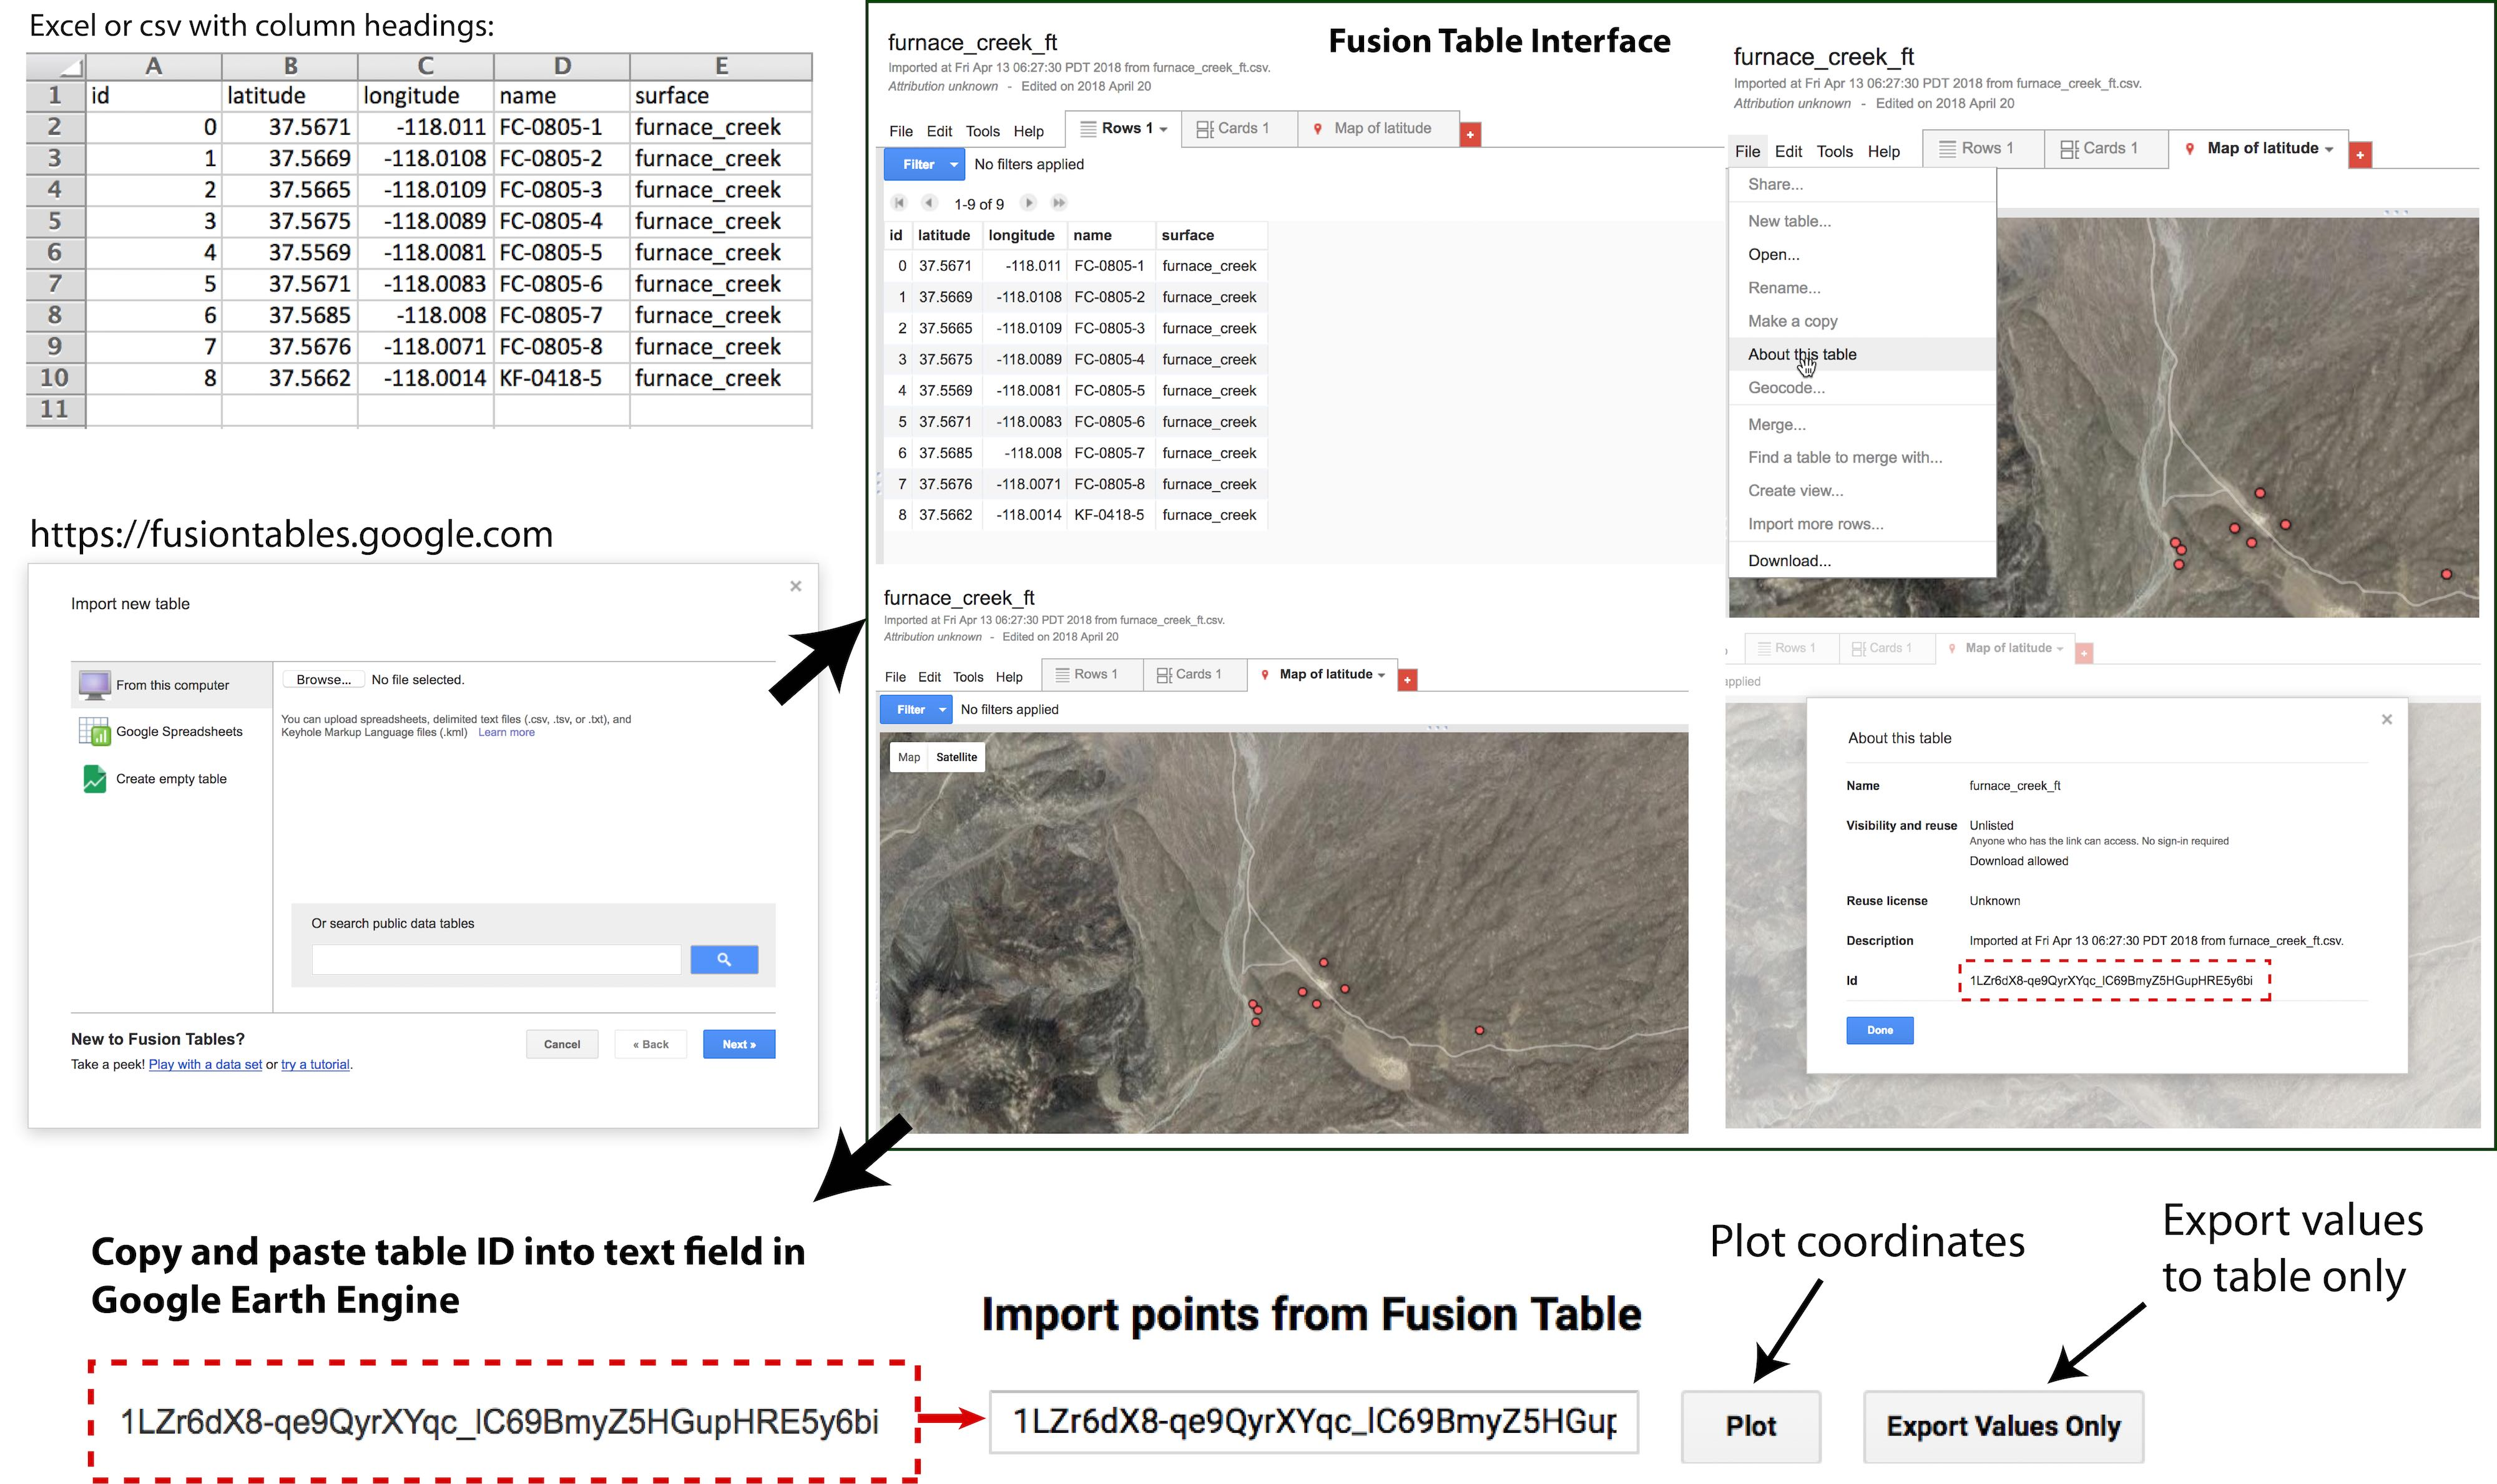
\includegraphics[width=1.2\textwidth,keepaspectratio]{images/fusion_table_reduced.jpg}
\caption{Importing coordinate, name and surface data for predefined points can be achieved effectively using the above .csv format (top left), which can then be uploaded into Google's fusion table service (\href{https://fusiontables.google.com}{fusiontables.google.com}). The column names are both case-sensitive and fixed, the ``id'' column is simple a incremental unique identifier (0 ... nth item), ``latitude'' and ``longitude'' are decimal coordinate values in WGS84, ``name'' is the string id for a give point and ``surface'' is a grouping variable, enabling a single fusion table to contain a number of different sample groups. An example fusion table can be seen in the larger top right panel, with a capability to preview the location of data points in a separate mapping viewport. Crucially, the ID of the fusion table is found in the \textit{File >> About this table window}, which is the hash string required to input into the ``Fusion table ID'' text box in \textit{Spectal Point}. Once inputted, the user can either plot all the points in the table, which can be a slow process for over points, or simply export pixel values to a .csv file in their Google Drive (Bottom row).}
\label{fig:fusion_table}
\end{figure}
\end{landscape}

\section{Exporting Data}
\label{export-data}
With a selection of query points, the data that can be exported from \textit{Spectral Point} includes a tabulated series of reflectance values across each selected band and a KMZ file containing the position of each query point (See figure~\ref{fig:export}). Each exported file is saved as a task in a GEE submenu that the user must activate to begin processing and storage in the user's Google Drive (See figure~\ref{fig:export_task}).

\begin{figure}[htbp]
\centering
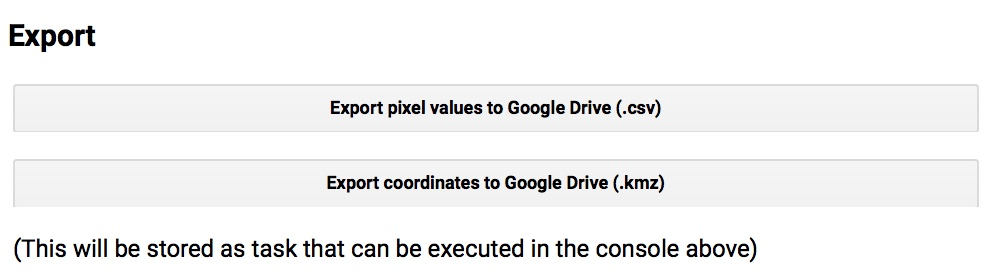
\includegraphics[width=1.0\textwidth]{images/export.jpeg}
\caption{Two data export options are available to the user, the top button exports all query point pixel  values across all bands, including PCA bands if they have been processed. The data that is exported to the Google Drive will be a text-delimited .csv file. The lower button will export the coordinates of each point a compressed Keyhole Markup Language (.kmz) file for viewing in Google Earth Pro or other desktop GIS applications. No band data is exported in the .kmz file.}
\label{fig:export}
\end{figure}

\begin{figure}[htbp]
\centering
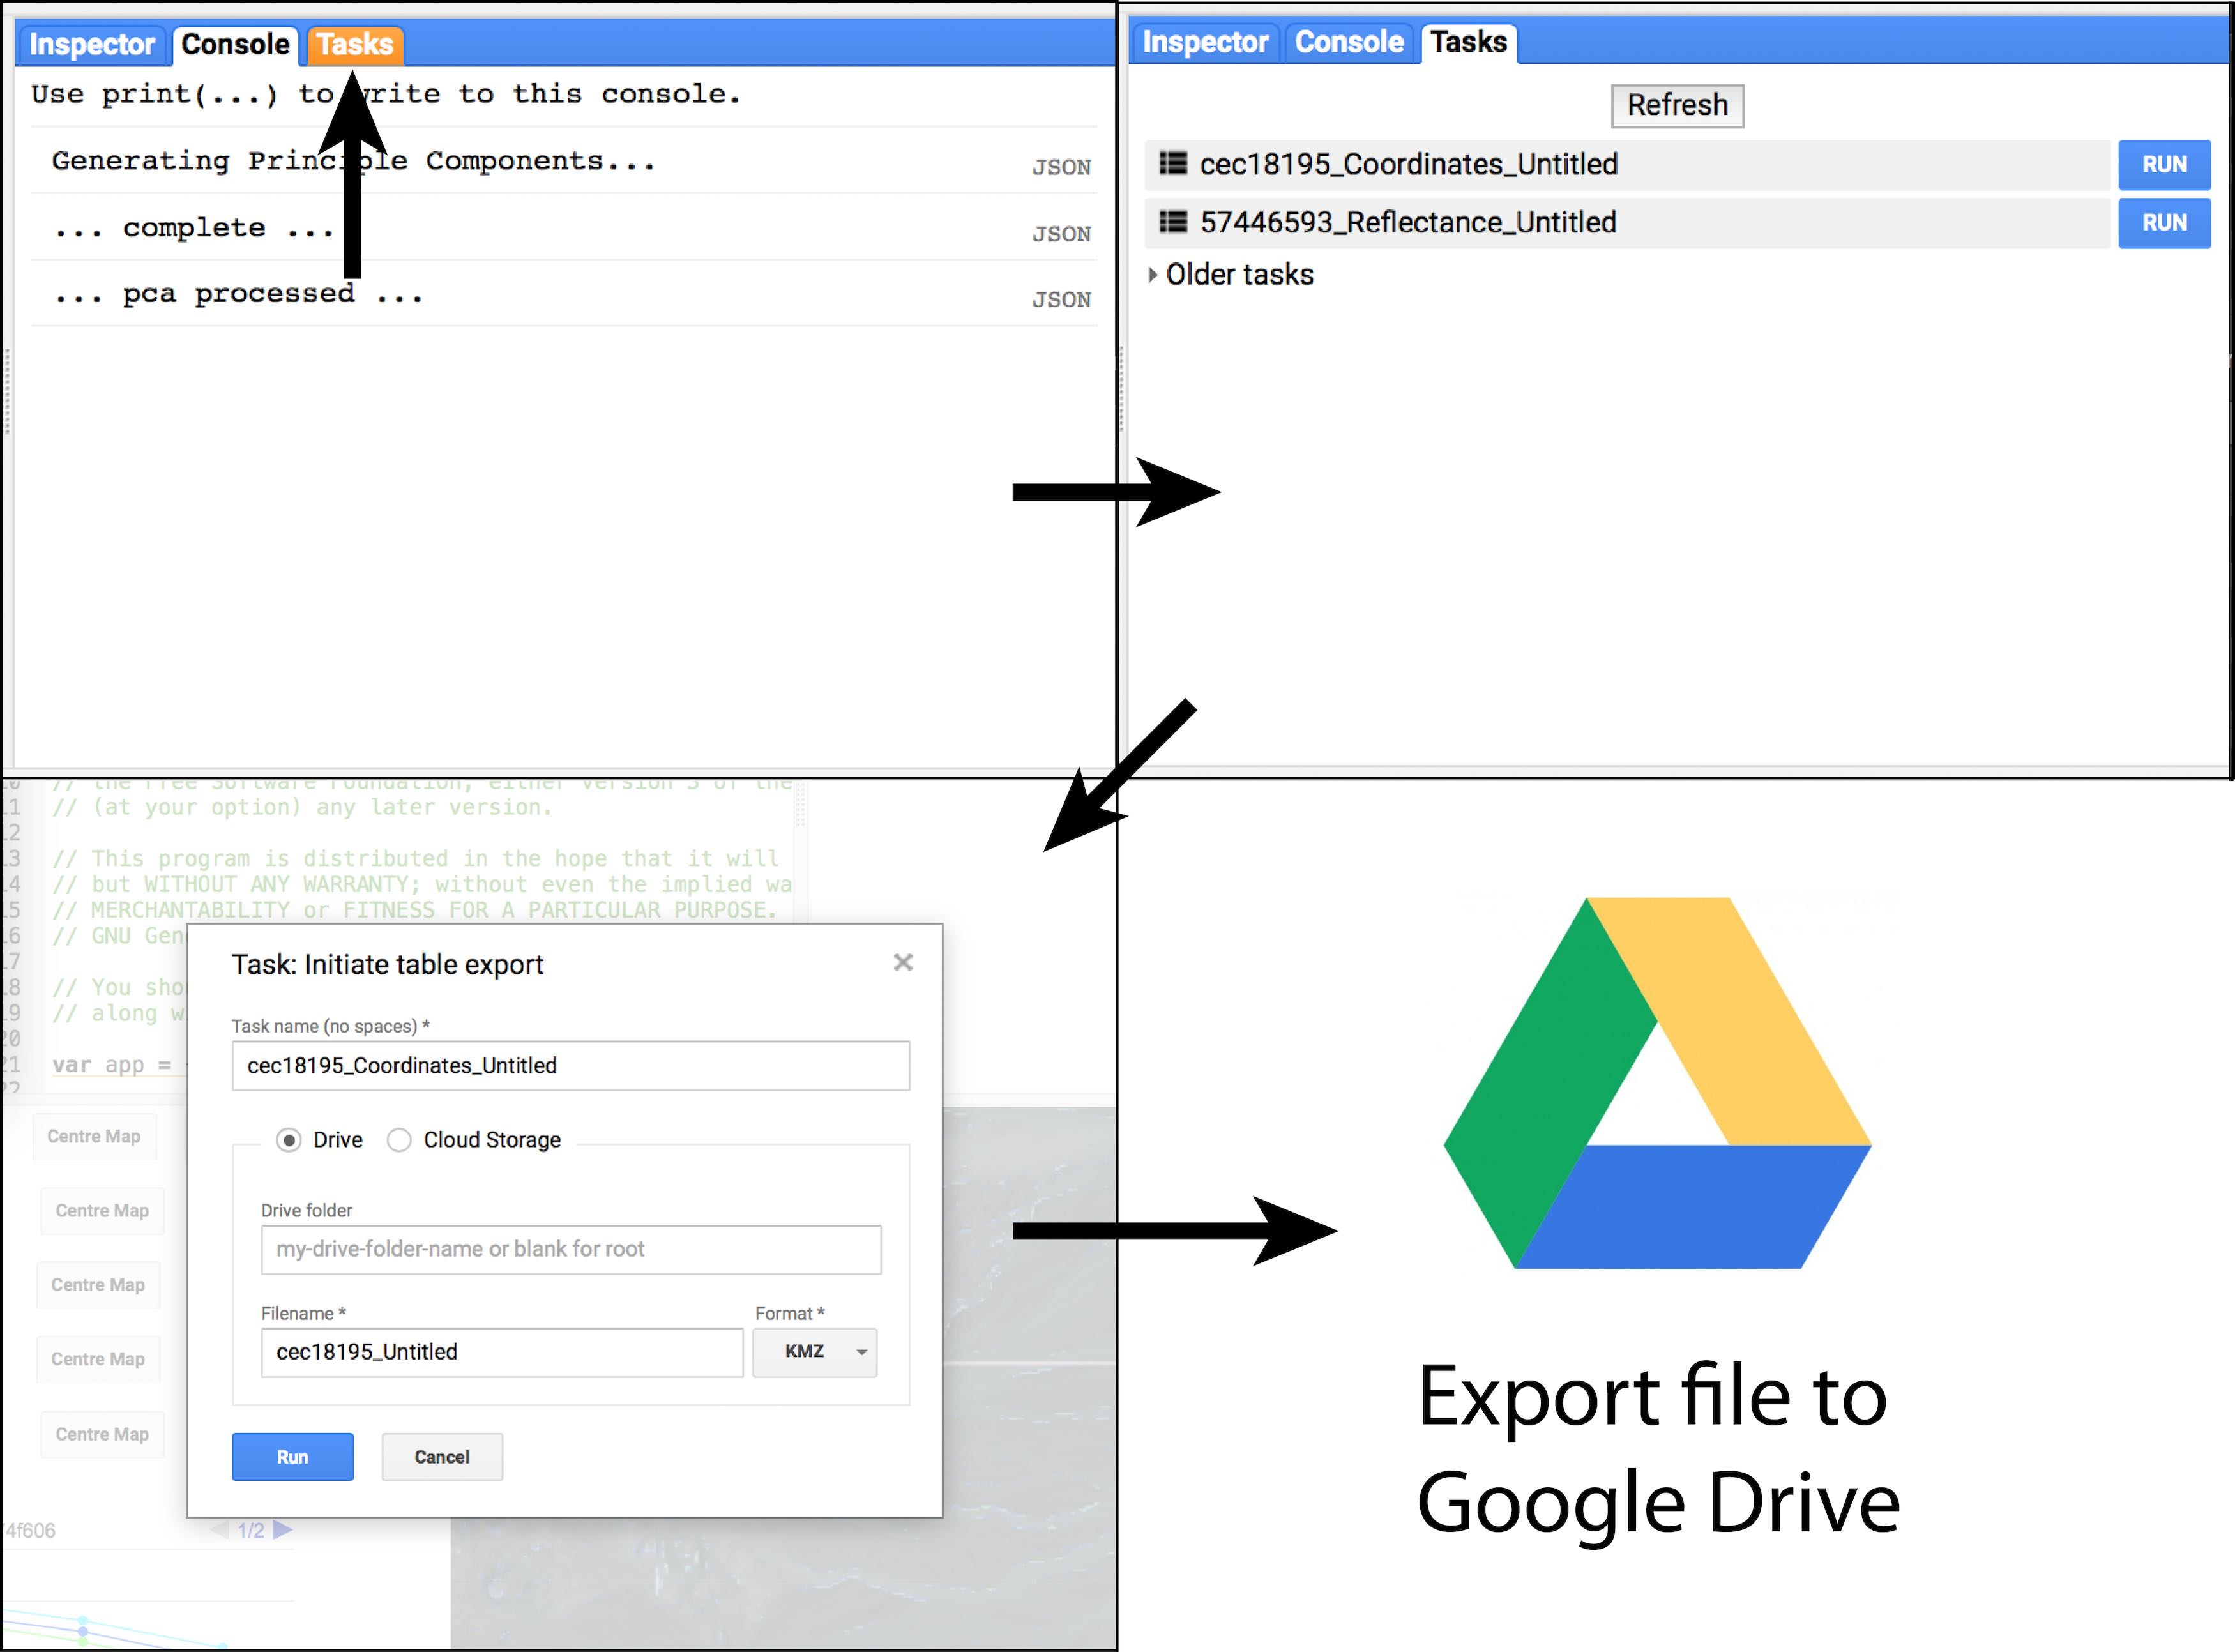
\includegraphics[width=1.0\textwidth]{images/export_task_reduced.jpg}
\caption{Exporting data from \textit{Spectral Point} is achieved using GEE's export facility to a user's corresponding Google Drive. When either of the two buttons in figure~\ref{fig:export} are pressed, the task tab in the console window (See~\ref{fig:workspace_fig}) will light up, as seen in the top left panel. The top right panel shows two new tasks that have yet to be initiated. Only when the user clicks ``Run'', will the export task be carried out, with several options to change the name and destination, seen in the bottom left panel. Processing time can take anywhere from seconds to minutes, and if will fail if memory limits are exceeded.}
\label{fig:export_task}
\end{figure}

\section{Further Information}

{

\textbf{The Landsat Project}\\
\href{https://landsat.usgs.gov/}{landsat.usgs.gov}

\textbf{Google Earth Engine Development}\\
\href{https://developers.google.com/earth-engine/}{developers.google.com/earth-engine}

\textbf{Image Processing - Liu and Mason, 2009}\\
\href{https://doi.org/10.1002/9781118724194}{doi.org/10.1002/9781118724194}

\textbf{Principal Component Analysis - Simplified}\\
\href{http://setosa.io/ev/principal-component-analysis/}{setosa.io/ev/principal-component-analysis}
}

\begin{footnotesize}
\singlespacing
\bibliographystyle{apalike}
\bibliography{bibliography}
\end{footnotesize}

\end{document}  
